\chapter{Conceptos Preliminares}

    %\thispagestyle{empty}

    \lettrine[lines=5] { \initfamily \selectfont E}{s} imposible estudiar una teoría matemática sin antes establecer sus definiciones básicas y su notación respectiva. En este capítulo desglosaremos brevemente las ideas y la terminología de las dos ramas de las Matemáticas involucradas en esta tesis. Muchos de los resultados mencionados aquí los dejaremos sin demostración ya que no es nuestro objetivo principal.
    
 

        \section{Álgebra Lineal}
        A continuación abordaremos los conceptos y las notaciones de las que haremos uso a lo largo de este trabajo. Si el lector está interesado en profundizar en estos temas, y desea conocer las demostraciones de los teoremas mencionados, se le invita a revisar \cite{Friedberg,Noble,Zhang, Shores}.

        \subsection{¿Qué es un espacio vectorial?}
            Un \textit{campo}\index{Campo} $\mathbb{F}$ es un conjunto, en el cual están definidas dos operaciones  $+$ y $\bullet$, llamadas \textit{suma} y \textit{multiplicación}, respectivamente, de tal manera que por cada par de elementos $x,y \in \mathbb{F}$, existen únicos $x+y$ y $x \bullet y$ en $\mathbb{F}$. Además, para todo $a,b,c \in \mathbb{F}$, deben cumplirse las siguientes condiciones\index{Campo! propiedades de}: 
                \begin{enumerate}
                    \item \textit{Conmutatividad de la suma y multiplicación}:
                        $a + b = b + a$  y  $a \bullet b = b \bullet a$
                    \item \textit{Asociatividad de la suma y multiplicación}:
                        $(a + b) + c = a + (b + c)$  y  $(a \bullet b)\bullet c = a\bullet(b \bullet c)$.
                    \item \textit{Existencia del neutro aditivo y del neutro multiplicativo}:
    
                        Existen  $0, 1 \in\mathbb{F}$, tales que:
                         $0 + a = a$  y  $1 \bullet a = a$.
    
                    \item \textit{Existencia del inverso aditivo y del inverso multiplicativo}:
    
                        Para cualesquiera $a$ en $\mathbb{F}$ y  $b \neq 0$ en $\mathbb{F}$, existen $c$ y $d$ en $\mathbb{F}$ tales que:
                        $a + c  =  0$  y  $b \bullet d  =  1$.
                        
                    \item \textit{Distributividad de la multiplicación sobre la suma}:
                        $a \bullet(b + c)  = a \bullet b  +  a \bullet c$
                 \end{enumerate}

            El campo más sencillo con el que trabajaremos en esta tesis es el campo de Galois $GF(2)$ (también denotado por $\mathbb{Z}_{2}$ ó $\mathbb{F}_{2}$). Este campo es el conjunto $\{0,1\}$ con las operaciones dadas por las siguientes tablas (puede notarse que aquí la suma coincide con el álgebra módulo $2$ en los números enteros):

            \begin{center}
                \begin{tabular}{ c | c c }
                    + & 0 & 1 \\ \hline
                    0 & 0 & 1 \\  
                    1 & 0 & 0    
                \end{tabular}
            \end{center}

            \begin{center}
                \begin{tabular}{ c | c c }
                    $\bullet$ & 0 & 1 \\ \hline
                    0 & 0 & 0 \\  
                    1 & 0 & 1    
                \end{tabular}
            \end{center}

            Otros campos más utilizados son los números reales $\mathbb{R}$ y los complejos $\mathbb{C}$ con la suma y multiplicación usuales.


            Un \textit{espacio vectorial $V$ sobre un campo $\mathbb{F}$}\index{Espacio! vectorial} consiste de un conjunto $V$ con dos operaciones definidas en él, llamadas  \textit{suma} $+$ y \textit{multiplicación escalar} $\cdot$, tales que, para cualesquiera $\mathbf{x,y} \in V$ y todo $k \in \mathbb{F}$, existen únicos $\mathbf{x + y} \in V$ y $k \cdot \mathbf{x} \in V$. Además, estas operaciones deben cumplir lo siguiente:
 
            \begin{enumerate}
                \item Para cualesquiera $\mathbf{x,y} \in V$, $\mathbf{x + y = y + x}$.
                \item Para cualesquiera $\mathbf{x,y,z} \in V$, $\mathbf{(x+y)+z = x+ (y+z)}$.
                \item Existe un elemento $\mathbf{0} \in V$ tal que, para todo $\mathbf{x} \in V$, $\mathbf{x + 0 = x}$.
                \item Para todo $\mathbf{x} \in V$, existe $\mathbf{-x} \in V$ tal que $\mathbf{x + (-x) = 0}$.
                \item Para todo $\mathbf{x}$, $1 \cdot \mathbf{x} = \mathbf{x}$.
                \item Para cualesquiera $a,b \in \mathbb{F}$, y todo $\mathbf{x} \in V$, $(ab)\cdot \mathbf{x} = a(b\cdot\mathbf{x})$.
                \item Para todo $a \in \mathbb{F}$, y cualesquiera $\mathbf{x,y}$, $a \cdot (\mathbf{x + y}) = a\cdot \mathbf{x} + a\cdot \mathbf{y}$.
                \item Para cualesquiera $a,b \in \mathbb{F}$, y todo $\mathbf{x}$, $(a+b) \cdot (\mathbf{x}) = a\cdot \mathbf{x} + b\cdot \mathbf{x}$.
            \end{enumerate}
 
            A los elementos de $\mathbb{F}$ y $V$ les llamamos \textit{escalares}\index{Escalar} y \textit{vectores}\index{Vector}, respectivamente. Un subconjunto $W$ de un espacio vectorial $V$ sobre $\mathbb{F}$ es un \textit{subespacio vectorial}\index{Espacio! subespacio} si $W$ es un espacio vectorial sobre $\mathbb{F}$ con las mismas operaciones definidas en $V$. De hecho, se sabe que $W$ es un subespacio si  y sólo si $\mathbf{0} \in W$, $\mathbf{x + y} \in W$, para cualesquiera $\mathbf{x,y} \in W$; y $k\mathbf{x} \in W$, para todo $k \in \mathbb{F}$ y $\mathbf{x} \in W$. 
            
            Una $n-$ada ordenada es un vector del espacio $\mathbb{F}^{n}$ y la escribimos en \textit{forma de columna}. Así, dados $a_{1}, \ldots, a_{n} \in \mathbb{F}$, escribimos 
                $$
                \begin{bmatrix}
                    a_{1} \\
                    \vdots \\
                    a_{n}
                \end{bmatrix} \in \mathbb{F}^{n}.
                $$

            Dependiendo de la situación, estas $n-$adas se escribirán en \textit{forma de renglón}:$\begin{bmatrix}
                    a_{1} & \cdots & a_{n}
                \end{bmatrix}$. Si agregamos el superíndice ``$\textnormal{T}$'' al \textit{vector renglón}\index{Vector!renglón}, entonces obtenemos un \textit{vector columna}\index{Vector! columna}, es decir:
                $$
                \begin{bmatrix}
                    a_{1} & \cdots & a_{n}
                \end{bmatrix} ^{\textnormal{T}} = \begin{bmatrix}
                    a_{1} \\
                    \vdots \\
                    a_{n}
                \end{bmatrix}. 
                $$

            Resulta que $\mathbb{F}^{n}$ es uno de los espacios vectoriales más conocidos, cuya suma y producto escalar se hacen \textit{entrada a entrada} con la suma y producto del campo $\mathbb{F}$. En efecto, sean $\begin{bmatrix} a_{1} & \cdots & a_{n}\end{bmatrix} ^{\textnormal{T}}$ y $\begin{bmatrix} b_{1} & \cdots & b_{n} \end{bmatrix} ^{\textnormal{T}}$ en $\mathbb{F}^{n}$ y $k \in \mathbb{F}$. Entonces
                $$
                \begin{bmatrix}
                a_{1} \\
                \vdots \\
                a_{n}
                \end{bmatrix} + \begin{bmatrix}
                b_{1} \\
                \vdots \\
                b_{n}
                \end{bmatrix}  =\begin{bmatrix}
                a_{1} + b_{1} \\
                \vdots \\
                a_{n} + b_{n}
                \end{bmatrix} \in \mathbb{F}^{n}
                $$ y $$ k \cdot\begin{bmatrix}
                a_{1} \\
                \vdots \\
                a_{n}
                \end{bmatrix} = \begin{bmatrix}
                ka_{1} \\
                \vdots \\
                ka_{n}
                \end{bmatrix} \in \mathbb{F}^{n}.$$

            De lo anterior, se desprende que  $\mathbb{R}^{n}$ y $\mathbb{C}^{n}$ también  son espacios vectoriales. Si $\mathbb{F} = GF(2)$, entonces denotamos por $\oplus$ a la suma en $GF(2)^{n}$. Ésta, desde luego, se hace entrada a entrada siguiendo las operaciones que exhibimos en tablas líneas arriba. Por ejemplo, tomemos $\begin{bmatrix} 1 & 0 & 1 & 1 \end{bmatrix}^{\textnormal{T}}$ y $\begin{bmatrix} 0 & 1 & 1 & 1 \end{bmatrix}^\textnormal{T}$ en $GF(2)^{4}$. Entonces 
                $$ \begin{bmatrix}
                1 \\
                0 \\
                1\\
                1
                \end{bmatrix} \oplus \begin{bmatrix}
                0 \\
                1\\
                1\\
                1
                \end{bmatrix}  =\begin{bmatrix}
                1 \\
                1 \\
                0\\
                0
                \end{bmatrix}.
                $$


        \subsection{Combinaciones lineales e independencia lineal}
%XXXXXXXXXXXXXXXXXXXXXXX****¡¡REVISADO!!****XXXXXXXXXXXXXXXXXXXXXXXX
%XXXXXXXXXXXXXXXXXXXXXXX****¡¡REVISADO!!****XXXXXXXXXXXXXXXXXXXXXXXX
%XXXXXXXXXXXXXXXXXXXXXXX****¡¡REVISADO!!****XXXXXXXXXXXXXXXXXXXXXXXX        
            Dados un  espacio vectorial $V$ y $S \subseteq V$, decimos que $\mathbf{v} \in V$ es una \textit{combinación lineal de vectores de $S$} \index{Combinación lineal} si existe una cantidad finita de vectores $\mathbf{u_{1}, \ldots, u_{n}} \in S$ y escalares $k_{1}, \ldots, k_{n}\in \mathbb{F}$ tales que $\mathbf{v} = k_{1}\mathbf{u}_{1} + \cdots + k_{n}\mathbf{u}_{n}$. Usualmente llamamos \textit{coeficientes} a los escalares de la combinación lineal.

            El conjunto de todas las posibles combinaciones lineales de vectores en $S$ es llamado el \textit{espacio generado de $S$}\index{Espacio! generado} y lo escribimos $span(S)$ y es un subespacio de $V$. Si $span(S) = V$, se dice que $S$ \textit{genera} a $V$.

            Si hacemos una combinación lineal $k_{1}\mathbf{u}_{1} + \cdots +k_{n}\mathbf{u}_{n} = \mathbf{0} $, con $k_{1} = \ldots= k_{n} = 0$, entonces ésta es llamada \textit{combinación lineal trivial del} $\mathbf{0}$. Un conjunto de vectores $S$ se dice que es \textit{linealmente dependiente} \index{Linealmente! dependiente}si existe una combinación lineal del $\mathbf{0}$ no trivial con vectores de $S$. En caso contrario, esto es, cuando la única combinación lineal del $\mathbf{0}$ es la trivial, se dice que $S$ es un conjunto \textit{linealmente independiente}\index{Linealmente! independiente}.

            Se sabe que si $S \subseteq T$ y $T$ es linealmente independiente, entonces $S$ es también linealmente independiente. Si $S$ es linealmente dependiente, necesariamente $T$ también lo es. De igual modo, se conoce que, si $\mathbf{u} \notin S$, entonces $S\cup \{\mathbf{u}\}$ es linealmente dependiente si y sólo si $\mathbf{u} \in span(S)$.

            Una \textit{base}\index{Base} $\beta$ de $V$ es un subconjunto linealmente independiente de $V$ tal que $span(\beta) = V$. Las bases de los espacio vectoriales son de suma importancia. Por ejemplo, todo vector de $V$ puede expresarse de manera única como combinación lineal de vectores de $\beta$ y cualesquiera de sus bases tienen la misma cardinalidad. Este número es la \textit{dimensión}\index{Dimensión} del espacio vectorial y se le denota como $\dim(V)$. En particular, todos los espacios que trataremos en esta tesis son de \textit{dimensión finita}.

            Una base de $\mathbb{F}^{n}$ es aquella conformada por los vectores canónicos $\mathbf{e}_{i}$ (cuya $i-$ésima entrada es $1$ y $0$ en las demás). Por lo que $\dim(\mathbb{F}^{n}) = n$.

            Si $W$ es un subespacio de $V$, entonces $\dim(W) \leq \dim(V)$. La cantidad de elementos en un conjunto linealmente independiente no puede exceder la dimensión del espacio. Tampoco el número de vectores en un conjunto generador es menor que dicha dimensión. En otras palabras, si $S$ es linealmente independiente en $V$ y $span(T)=V$, entonces $|S| \leq \dim(V) \leq |T|$.

            Dados $A$ y $B$ subespacios de $ V$, la suma \index{Suma! de dos subespacios} de $A$ y $B$ es el subespacio $$A+B := \{ \mathbf{x + y} \in V\ | \mathbf{x}\in A, \mathbf{y} \in B \}.$$
            
            Decimos que $V$ \textit{es suma directa de} $A$ y $B$ si y sólo si $A \cap B= \{\mathbf{0}\}$ y $A+B = V$. Si ocurre lo anterior, escribimos $V = A \oplus B$ y se cumple que $\dim(V) = \dim(A) + \dim(B)$. Además, si $\beta_{1}$ y $\beta_{2}$ son bases de $A$ y $B$, respectivamente, entonces $\beta_{1} \cup \beta_{2}$  es una base de $V$. Observe que esta última definición (junto con sus propiedades) se pueden extender a cualquier cantidad de subespacios vectoriales. 
            %\vspace{-0.15cm}
            
        \subsection{Transformaciones lineales}
%XXXXXXXXXXXXXXXXXXXXXXX****¡¡REVISADO!!****XXXXXXXXXXXXXXXXXXXXXXXX
%XXXXXXXXXXXXXXXXXXXXXXX****¡¡REVISADO!!****XXXXXXXXXXXXXXXXXXXXXXXX
%XXXXXXXXXXXXXXXXXXXXXXX****¡¡REVISADO!!****XXXXXXXXXXXXXXXXXXXXXXXX          
            Las transformaciones lineales entre espacios vectoriales son una clase especial de funciones que preservan la estructura de los espacios. En \cite{Friedberg} hay un estudio extenso sobre ellas. Formalmente, si $V$ y $W$ son espacios vectoriales (ambos  sobre $\mathbb{F}$), una función $T : V \rightarrow W$ es una \textit{transformación lineal}\index{Transformación lineal} si para cualesquiera $\mathbf{x,y} \in V$ y todo $ c \in \mathbb{F}$, se cumple que $T(\mathbf{x + y}) = T(\mathbf{x}) + T(\mathbf{y})$ y $T(c\mathbf{x}) = c\cdot T(\mathbf{x})$.


            Hay dos subespacios vectoriales asociados a una transformación $T$: el \textit{Kernel}\index{Kernel! de una transformación} (o \textit{núcleo}) de $T$, que es el conjunto $Ker(T):= \{ \mathbf{x} \in V | T(\mathbf{x}) = \mathbf{0}\}$; y la \textit{imagen} \index{Imagen de una transformación} de $T$, que es $Im(T):= \{ T(\mathbf{x}) | \mathbf{x} \in V\}$. El \textit{rango} de $T$ \index{Rango de una transformación} es la dimensión de su imagen y la \textit{nulidad} \index{Nulidad! de una transformación} de $T$ es la dimensión de su kernel, es decir,
                \begin{align*}
                rank(T)&:= \dim(Im(T)),\\ 
                null(T)&:= \dim(Ker(T)).
                \end{align*}
            El \textit{teorema de la dimensión} (o \textit{teorema de rango-nulidad}) establece que, si $V$ tiene dimensión finita, entonces $\dim(V)= rank(T) + null(T)$.

            Decimos que dos espacios $V$ y $W$ son \textit{isomorfos} \index{Isomorfismo} si y sólo si existe una transformación lineal biyectiva $T \colon V \rightarrow W$. A tal transformación se le llama \textit{isomorfismo}. Importantes teoremas se deducen de esta definición: si dos espacios son isomorfos, entonces tienen la misma dimensión; aún más, si $V$ es un espacio vectorial sobre $\mathbb{F}$ y $\dim(V) =n$, entonces $V$ es isomorfo a $\mathbb{F}^{n}$.


        \subsection{Ortogonalidad}
%XXXXXXXXXXXXXXXXXXXXXXX****¡¡REVISADO!!****XXXXXXXXXXXXXXXXXXXXXXXX
%XXXXXXXXXXXXXXXXXXXXXXX****¡¡REVISADO!!****XXXXXXXXXXXXXXXXXXXXXXXX
%XXXXXXXXXXXXXXXXXXXXXXX****¡¡REVISADO!!****XXXXXXXXXXXXXXXXXXXXXXXX        
            Un espacio vectorial sobre el campo $\mathbb{F}=\mathbb{R}$ (ó $\mathbb{F}=\mathbb{C}$) es un \textit{espacio con producto interior}\index{Espacio! con producto interior} si está dotado de un \textit{producto interior} $\langle \cdot{,} \cdot \rangle$ (también llamado \textit{producto escalar} o \textit{producto interno})\index{Producto interior} que satisface, para todo $k \in \mathbb{F}$ y para cualesquiera $\mathbf{u,v,w} \in V$, lo siguiente:
                \begin{enumerate}
                    \item $\langle \mathbf{u,u}\rangle \geq 0$ y $\langle \mathbf{u,u}\rangle = 0$ si y sólo si $\mathbf{u} = \mathbf{0}$.
                    \item $\langle \mathbf{u+v,w} \rangle = \langle \mathbf{u,w} \rangle + \langle \mathbf{v,w}\rangle$.
                    \item $ \langle k\mathbf{u,v}\rangle =  k\langle \mathbf{u,v}\rangle$.
                    \item $\overline{ \langle \mathbf{u,v}\rangle} =  \langle \mathbf{v,u}\rangle$.
                \end{enumerate}


            Al tener un producto interior definido en $V$, obtenemos una noción de \textit{ortogonalidad} entre vectores. De hecho, se dice que dos vectores $\mathbf{x,y} \in V$ son ortogonales si y sólo si $ \langle \mathbf{x,y}\rangle =0$.\index{Vectores ortogonales} Si $S$ es un subconjunto no vacío de $V$, entonces el \textit{complemento ortogonal de}\index{Complemento ortogonal} $S$ es el subespacio $S^{\perp}$ de vectores ortogonales a todo vector de $S$, o sea, $$S^{\perp}:= \{\mathbf{x} \in V |  \langle \mathbf{x,y}\rangle = 0, \textnormal{para todo } y \in S\}.$$
            
            Dados $\mathbf{x,y} \in \mathbb{R}^{n}$, el producto interior usual en $\mathbb{R}^{n}$ es $$ \langle \mathbf{x,y}\rangle := \sum_{i = 1}^{n} x_{i}y_{i}.$$
            
            Para espacios vectoriales sobre campos finitos, como $GF(2)$, también podemos considerar el mismo producto interior usual. No obstante, como se verá más adelante, este producto escalar (en espacios sobre campos finitos) falla en el primer punto de la definición de producto interno: hay vectores $\mathbf{u}$ tales que $\langle \mathbf{u,u}\rangle = 0$ pero $\mathbf{u}\neq \mathbf{0}$. Entonces hay vectores \textit{ortogonales a sí mismos}. Sólo se cumple que $\langle \mathbf{u},\mathbf{u}\rangle \geq 0$ y, si $\mathbf{u} = \mathbf{0}$, necesariamente $\langle \mathbf{u,u}\rangle = 0$. Los productos escalares que verifican esto último (en vez del punto 1 de la definición) se llaman \textit{productos interiores degenerados}. \index{Producto interior degenerado}

        \subsection{Matrices}
%XXXXXXXXXXXXXXXXXXXXXXX****¡¡REVISADO!!****XXXXXXXXXXXXXXXXXXXXXXXX
%XXXXXXXXXXXXXXXXXXXXXXX****¡¡REVISADO!!****XXXXXXXXXXXXXXXXXXXXXXXX
%XXXXXXXXXXXXXXXXXXXXXXX****¡¡REVISADO!!****XXXXXXXXXXXXXXXXXXXXXXXX           
            Una \textit{matriz} \index{Matriz}$\mathbf{A}$ \textit{de} $n \times m$ \textit{sobre un campo} $\mathbb{F}$ es un arreglo rectangular de  $m$ renglones y $n$ columnas. El conjunto de estas matrices se escribe como $\mathbb{M}_{n \times m}(\mathbf{F})$. Los vectores columna de $n$ entradas, en particular, se pueden considerar como matrices de tamaño $1 \times n$.  La matriz cuyas entradas son todas $0$ se escribe $\mathbf{O}$ y frecuentemente escribimos $\mathbf{A} = [a_{ij}]$ para denotar, de manera abreviada, a la matriz $\mathbf{A}$ y sus entradas, es decir,
                $$
                \mathbf{A}:= \begin{bmatrix}
                a_{11} & \cdots & a_{1m}\\ 
                \vdots & \ddots &\vdots\\ 
                a_{n1} &\cdots  & a_{nm} 
                \end{bmatrix}.
                $$
                
            Definimos la $j-$ésima \textit{columna de}  $\mathbf{A}$ como el vector de tamaño $n \times 1$ $$\mathbf{c}_{j} := \begin{bmatrix}
            a_{1j} \\ 
            \vdots\\
            a_{nj}
            \end{bmatrix}
            $$ Entonces escribimos $\mathbf{A} = \begin{bmatrix}
            \mathbf{c}_{1} | & \cdots & |\mathbf{c}_{m}
            \end{bmatrix}.$  Análogamente, el $i-$ésimo \textit{renglón} de $\mathbf{A}$ es el vector de tamaño $1 \times n$, $\mathbf{r}_{i}:= \begin{bmatrix}
            a_{i1} & \cdots & a_{im}
            \end{bmatrix}.$ Y escribimos: $$\mathbf{A} = \begin{bmatrix}
            \mathbf{r}_{1}\\
            \--\\
            \vdots \\
            \--\\
            \mathbf{r}_{n}
            \end{bmatrix}.$$ Démonos cuenta que $\mathbf{c}_{j} \in \mathbb{F}^{n}$ y $\mathbf{r}_{i} \in \mathbb{F}^{m}$.    

          
            La suma \index{Suma de matrices} de dos matrices del mismo tamaño, $\mathbf{A} = [a_{ij}]$ y $\mathbf{B} = [b_{ij}]$, es la matriz $\mathbf{A+B}: = [a_{ij} + b_{ij}]$. También definimos el producto de un vector renglón y un vector columna como sigue:
            
            Supongamos que $\mathbf{a}:=\begin{bmatrix}
            a_{1} & \cdots & a_{m}\\ 
            \end{bmatrix}$ y $\mathbf{b}:=\begin{bmatrix}
            b_{1} \\ 
            \vdots\\
            b_{m}\\ 
            \end{bmatrix}$. Entonces $$\mathbf{a}\mathbf{b} = \begin{bmatrix}
            a_{1} & \cdots & a_{m}\\ 
            \end{bmatrix} \begin{bmatrix}
            b_{1} \\ 
            \vdots\\
            b_{m}\\ 
            \end{bmatrix}:= [a_{1}b_{1} + \cdots + a_{m}b_{m}].$$

            
            De esta manera, dadas $\mathbf{A} \in \mathbb{M}_{n \times m}(\mathbb{F})$ y $\mathbf{B} \in \mathbb{M}_{m \times q}(\mathbb{F})$, el \textit{producto de $\mathbf{A}$ y $\mathbf{B}$} es la matriz $\mathbf{AB} \in \mathbb{M}_{n \times q}(\mathbb{F})$ de la forma $$ \mathbf{AB}:= \begin{bmatrix}
            \mathbf{r}_{1_{\mathbf{A}}}\mathbf{c}_{1_\mathbf{B}} | \cdots | \mathbf{r}_{m_{\mathbf{A}}}\mathbf{c}_{m_{\mathbf{B}}}
            \end{bmatrix}, $$ donde $\mathbf{r}_{i_\mathbf{A}}$ es el $i-$ésimo renglón de $\mathbf{A}$ y $\mathbf{c}_{i_\mathbf{B}}$ es la $i-$ésima columna de $\mathbf{B}$.
            
            
            El producto de una matriz de tamaño $n \times m$ por un vector de tamaño $m \times 1$ nos arroja otro vector de tamaño $n \times 1$. Dicho de otro modo, dado  $$\mathbf{x} = \begin{bmatrix}
            x_{1} \\
            \vdots \\
            x_{m}
            \end{bmatrix} \in \mathbb{F}^{m},$$ el producto $\mathbf{Ax}$ está dado por $$ \mathbf{Ax} =  \begin{bmatrix}
            \mathbf{c}_{1} | & \cdots & |\mathbf{c}_{m}
            \end{bmatrix} \begin{bmatrix}
            x_{1} \\
            \vdots\\
            x_{m}
            \end{bmatrix} = x_{1}\mathbf{c}_{1} + \cdots + x_{m}\mathbf{c}_{m} \in \mathbb{F}^{n}.
            $$
            
            El espacio generado por las columnas de $\mathbf{A}$ \index{Espacio! de columnas} lo denotamos como $\mathsf{C}(\mathbf{A})$; y al espacio generado por los renglones \index{Espacio! de renglones} lo escribimos como $\mathsf{R}(\mathbf{A})$. Al igual que las transformaciones lineales, las matrices también tienen un \textit{Kernel} (o \textit{espacio nulo})\index{Kernel! de una matriz} y es el conjunto $$Ker(\mathbf{A}) := \{\mathbf{x} \in \mathbb{F}^{m} | \mathbf{Ax} = \mathbf{0}\}.
            $$
            
            Estos espacios vectoriales nos permiten definir el rango y la nulidad de una matriz. En efecto, el \textit{rango} \index{Rango! de una matriz} de $\mathbf{A}$ es $rank(\mathbf{A}):= \dim(\mathsf{C}(\mathbf{A}))$ y la \textit{nulidad} \index{Nulidad! de una matriz} de $\mathbf{A}$ es $null(\mathbf{A}):= \dim(Ker(\mathbf{A}))$.
            
            Puede probarse que $rank(\mathbf{A})= \dim(\mathsf{R}(\mathbf{A}))$. Entonces, dados los conocimientos de espacios vectoriales y sus dimensiones, suele decirse que el rango de una matriz es \textit{el máximo número de sus columnas linealmente independientes} o \textit{el máximo número de sus renglones linealmente independientes}. Otra propiedad importante es  que $(\mathsf{R}(\mathbf{A}))^{\perp} = Ker(\mathbf{A})$ y $(Ker(\mathbf{A}))^{\perp} = \mathsf{R}(\mathbf{A})$.
            
             Si las columnas y renglones de una matriz $\mathbf{B}$ están contenidas en las columnas y renglones de $\mathbf{A}$, entonces decimos que $\mathbf{B}$ es \textit{submatriz}\index{Submatriz} de $\mathbf{A}$. 
            
             Una matriz $\mathbf{A}$ puede \textit{partirse}\index{Matriz! partición por bloques} en varias submatrices. Por ejemplo, $\mathbf{A}$ puede escribirse de la forma $$\mathbf{A} = \begin{bmatrix}
            \mathbf{B} & \mathbf{C} \\
            \mathbf{I} & \mathbf{O}
            \end{bmatrix}.$$ 
            
            En tal caso, se dice que $\mathbf{A}$ tiene una \textit{partición por} \textit{bloques}. Si $\mathbf{A}$ es de la forma $$\mathbf{A} = \begin{bmatrix}
            \mathbf{A}_{1} & \cdots & \mathbf{O} \\
            \vdots & \ddots & \vdots \\
            \mathbf{O} & \cdots & \mathbf{A}_{n}
            \end{bmatrix}$$ (donde, para todo $i\in\{1,\ldots,n\}$ $\mathbf{A}_{i}$ es submatriz de $\mathbf{A}$), decimos que $\mathbf{A}$ es una \index{Matriz! diagonal por bloques} \textit{matriz diagonal por bloques}. Entonces podemos probar que $\mathsf{C}(\mathbf{A}) = \mathsf{C}(\mathbf{A}_{1})\oplus \cdots \oplus \mathsf{C}(\mathbf{A}_{n})$ y también que $\mathsf{R}(\mathbf{A}) = \mathsf{R}(\mathbf{A}_{1})\oplus \cdots \oplus \mathsf{R}(\mathbf{A}_{n})$. Así, $rank(\mathbf{A}) = rank(\mathbf{A}_{1})+ \cdots + rank(\mathbf{A}_{n})$.
            
            Se dice que una matriz $\mathbf{A}$ es \textit{cuadrada} \index{Matriz! cuadrada} si tiene el mismo número de renglones que de columnas. Estas matrices poseen una gran relevancia en las aplicaciones del Álgebra Lineal. La \textit{diagonal} de una matriz cuadrada son sus entradas de la forma $a_{ii}$, con $i \in \{1, \ldots, n\}$; y se dice que $\mathbf{A}$ es una \index{Matriz! diagonal}\textit{matriz diagonal} si $a_{ij} = 0$ con $i\neq j$. En particular, la \textit{matriz identidad} \index{Matriz! identidad} $\mathbf{I}_{n}$ es aquella que en su diagonal tiene entradas iguales a $1$ y, en el resto, entradas iguales a $0$. 
            
            El \textit{determinante} \index{Determinante} es número que se asocia a las matrices cuadradas y otorga información relevante sobre dicha matriz. Dada $\mathbf{A} \in \mathbb{M}_{n \times n} (\mathbb{F})$, su determinante se calcula recursivamente mediante la \textit{fórmula de Laplace}:
            $$
            \det(\mathbf{A}):= \sum_{j=1}^{n} (-1)^{1+j} a_{1j} \det(\widetilde{\mathbf{A}}_{1j}),
            $$ donde $\widetilde{\mathbf{A}}_{1j}$ es la submatriz obtenida de $\mathbf{A}$ eliminando el renglón $1$ y la columna $j$.
            
            El estudio de las matrices es un campo bastante amplio. Si se quiere profundizar más al respecto, recordamos al lector que puede consultar  \cite{Friedberg,Noble,Zhang, Shores}.

        \section{Teoría de Gráficas}

        Para ser capaces de dar una definición satisfactoria de \textit{gráfica} (o \textit{grafo}) conviene primero recordar las siguientes definiciones. Dado un conjunto $A$, el conjunto de todos sus subconjuntos se le conoce como \textit{conjunto potencia de $A$} y se denota por $\mathcal{P}(A)$. Supongamos ahora que $A$ tiene $n$ elementos y tomemos $k \leq n$. Entonces $\binom{A}{k}$ es la familia de subconjuntos de $A$ cuya cardinalidad es $k$, esto es:
        $$ \binom{A}{k} = \Big\{ S \in \mathcal{P}(A) \Big| \: k = |S| \Big\} $$
        
        Gracias a la Combinatoria sabemos que $\left | \binom{A}{k} \right | = \binom{n}{k} = \frac{n!}{k! (n -k)!}$. Usualmente llamamos \textit{pares no ordenados} a los elementos de $\binom{A}{2}$ y de $\binom{A}{1}$.

        \subsection{Gráficas} \label{sec:queesunagrafica}

            Con lo comentado en los párrafos anteriores, decimos que una \textit{gráfica} \index{Gráfica} $G$ es un par ordenado $(V(G), E(G))$ que consiste de un conjunto $V(G)$ de \textnormal{vértices} \index{Vértice! de una gráfica} y un conjunto $E(G)$ de \textnormal{aristas}\index{Arista! de una gráfica} (ajeno con $V(G)$); junto con una \textnormal{función de incidencia} \index{Función de incidencia! de una gráfica }$\psi_{G} \colon E(G) \rightarrow \binom{V(G)}{1} \cup \binom{V(G)}{2}$ que asocia a cada arista de $G$ un par no ordenado de vértices de $G$ (no necesariamente distintos).Véase el ejemplo \ref{ejem:def}.

            Si $e$ es una arista y $u$ y $v$ son vértices de $G$ de tal manera que $\psi_{G}(e)=\{u,v\}$, entonces a $u$ y $v$ les llamamos \textit{extremos} \index{Vértice! extremo} de $e$. También es común decir que $e$ \textit{une} a los vértices $u$ y $v$, y que $u$ es adyacente a $v$ (y viceversa). De igual modo, cuando varias aristas comparten un extremo, decimos que tales aristas son adyacentes. \index{Vértices adyacentes} \index{Aristas adyacentes}
 
\begin{ejem} \label{ejem:def}
Sea $G=(V(G),E(G))$, con $V(G)=\{u_{1}, u_{2},u_{3},u_{4}\}$ y $E(G)=\{a,b,c,d,e,f\}$ y $\psi_{G}$ definida como sigue:

\begin{center}
\begin{tabular}{ c c c }
$\psi_{G}(a) = \{u_{1}\},$& $\psi_{G}(b) = \{u_{1},u_{2}\},$ & $\psi_{G}(c) = \{u_{2},u_{3}\},$  \\
$\psi_{G}(d) = \{u_{2},u_{4}\},$  & $\psi_{G}(e) = \{u_{3},u_{4}\},$  & $\psi_{G}(f) = \{u_{3},u_{4}\}.$ 
\end{tabular}
\end{center}

\hfill $\blacklozenge$
\end{ejem}
Es usual representar a las gráficas mediante \textit{diagramas} \index{Diagrama! de una gráfica} que nos ayudan a visualizar mucho mejor sus características. Estos diagramas consisten de \textit{puntos} y \textit{líneas} que simbolizan los vértices y las aristas, respectivamente. Un diagrama de este estilo muestra las relaciones de incidencia de forma sencilla. En la figura \ref{fig:diagrama} se muestra el diagrama de la gráfica del ejemplo \ref{ejem:def}.

\begin{figure}[h]
    \centering
    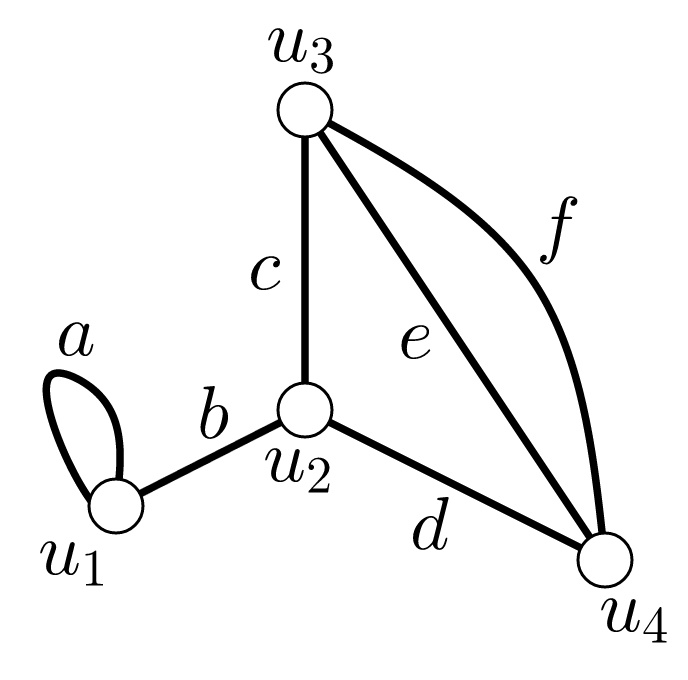
\includegraphics[scale=0.23]{img/imgchapter1/GrafoDefinicion.jpg}
    \caption{}
    \label{fig:diagrama}
\end{figure}

Es común referirse al diagrama como la gráfica en sí. Por tanto, los puntos del diagrama serán llamados también \textit{vértices} y sus líneas \textit{aristas}. La función de incidencia queda ya implícita, pues en el diagrama están claras las adyacencias entre vértices y aristas.

Para simplificar el discurso (y cuando no haya riesgo de ambigüedad), suele omitirse la letra ``$G$'' de los símbolos que usamos para denotar los conjuntos de vértices y aristas; así, escribimos ``$V$'' en vez de ``$V(G)$'' y ``$E$'' en lugar de ``$E(G)$''. También la función de incidencia queda sobreentendida.

Sea $G$ una gráfica y tomemos $e \in E$. Si sus extremos son iguales, se dice que $e$ es un \textit{lazo}\index{Lazo}. Si hay alguna otra arista, digamos $f$, con los mismos extremos que $e$, entonces decimos que $e$ y $f$ son \textit{aristas paralelas}\index{Arista! paralela}.
\begin{ejem}
En la gráfica de la figura \ref{fig:diagrama}, la arista $a$ es un lazo, pues $u_{1}$ es su único extremo. Mientras que las aristas $e$ y $f$ son paralelas, ya que $u_{3}$ y $u_{4}$ son sus extremos.

\hfill $\blacklozenge$
\end{ejem}
El \textit{grado de un vértice} \index{Grado de un vértice} es la cantidad total de aristas adyacentes en un vértice dado (los lazos se cuentan doble). A tal número se le denota por $d(v)$, y  $d_{G}(v)$ para enfatizar a qué gráfica pertenece el vértice $v$. Por ejemplo, basándonos en la figura \ref{fig:diagrama}, $d(u_{1})=3$ y $d(u_{4}) = 3$. Una de las propiedades más importantes de los grados es que \textit{la suma total de todos los grados de los vértices de una gráfica es, necesariamente, igual al doble del número de aristas en dicha gráfica}. En la sección \ref{sec:matriz} se dará una justificación de este hecho.

Decimos que $G$ es una \textit{gráfica simple}\index{Gráfica! simple} si no tiene lazos ni aristas paralelas. En tal caso, suele considerarse que $E(G) \subseteq V(G) \times V(G)$ (y la función de incidencia es la \textit{función inclusión de} $E(G)$). 

        \subsection{Tipos de gráficas} \label{sec:tiposdegraficas}
Una gráfica es \textit{finita} \index{Gráfica! finita}si sus conjuntos de vértices y aristas son finitos. Todas las gráficas que se estudian en este trabajo son finitas. Si estos conjuntos son vacíos, entonces la gráfica $(\emptyset, \emptyset)$ es \textit{nula}\index{Gráfica! nula}. 

Tomemos $n$ vértices (con $n\geq 1$), digamos $u_{1}, \ldots, u_{n}$ . La \textit{gráfica vacía} es la gráfica $$\varnothing := (\{u_{1}, \ldots, u_{n}\}, \emptyset),$$ es decir, $\varnothing$ es una gráfica que no tiene aristas. Si se quiere enfatizar el número de vértices de la gráfica vacía, entonces escribimos $\varnothing_{n}$. Si la gráfica consiste de un sólo vértice, decimos que es \textit{trivial}\index{Gráfica! trivial}. Cabe aclarar lo siguiente: cuando hablemos del \textit{conjunto vacío}, lo haremos utilizando el símbolo ``$\emptyset$''; por otro lado, el símbolo ``$\varnothing$'' representa a la gráfica vacía. El conjunto vacío y la gráfica vacía \textit{no} deben ser confundidos. 

Decimos que $H$ es \textit{subgráfica} \index{Subgráfica} de $G$ si $V(H) \subseteq V(G)$ y $E(H) \subseteq E(G)$ y $\psi_{H}$ es la \textit{restricción de} $\psi_{G}$ \textit{a} $E(H)$. Si lo anterior sucede, escribimos $H \subseteq G$. Una subgráfica de $G$ es \textit{generadora} \index{Gráfica!generadora} si su conjunto de vértices es exactamente el mismo que $G$, es decir, $H \subseteq G$ es \textit{generadora} si y sólo si $V(H)=V(G)$.

Sea $X \subseteq V(G)$. La \textit{subgráfica inducida por} \index{Gráfica! inducida} $X$, $G[X]$, es aquella cuyo conjunto de vértices es $X$ y sus aristas son aristas de $G$ que tienen sus extremos en $X$. Similarmente, si $S\subseteq E(G)$, $G[S]$ denota la \textit{subgráfica inducida por} $S$, cuyo conjunto de aristas es $S$ y su conjunto de vértices queda determinado por los extremos de las aristas en $S$. Para evitar confusiones, también decimos que $G[S]$ es una \textit{subgráfica inducida por aristas}. En particular, $G[S]$ es una \textit{subgráfica generadora inducida por aristas} si $S$ es su conjunto de aristas y conserva todos los vértices originales, es decir, su conjunto de vértices es $V(G)$.

Una \textit{gráfica completa} \index{Gráfica! completa}es una gráfica simple en la que cualesquiera dos vértices son adyacentes. Si tal gráfica consta de $n$ vértices, se le escribe como $K_{n}$. En el inciso $(a)$ de la figura \ref{fig:grafoscompletos} mostramos la gráfica completa de $5$ vértices.

Una \textit{gráfica bipartita}\index{Gráfica! bipartita} es una gráfica simple en la que su conjunto de vértices puede partirse en dos conjuntos, digamos $X$ y $Y$, de tal forma que cualquier arista tenga uno de sus extremos en $X$ y el otro en $Y$ (y, por tanto, que no haya aristas que unan dos vértices de $X$, ni tampoco de $Y$). Suele denotarse como $G[X,Y]$. 

Sea $G[X,Y]$ gráfica bipartita y supongamos que en $X$ y $Y$ hay $n$ y $m$ vértices, respectivamente. Si sucediera que todos los vértices de $X$ son adyacentes a todos los de $Y$, entonces decimos que $G[X,Y]$ es una \textit{gráfica bipartita completa}\index{Gráfica! bipartita completa} y se escribe $K_{n,m}$. En el inciso $(b)$ de la figura \ref{fig:grafoscompletos} está la gráfica $K_{3,2}$.

\begin{figure}[h]
    \centering
    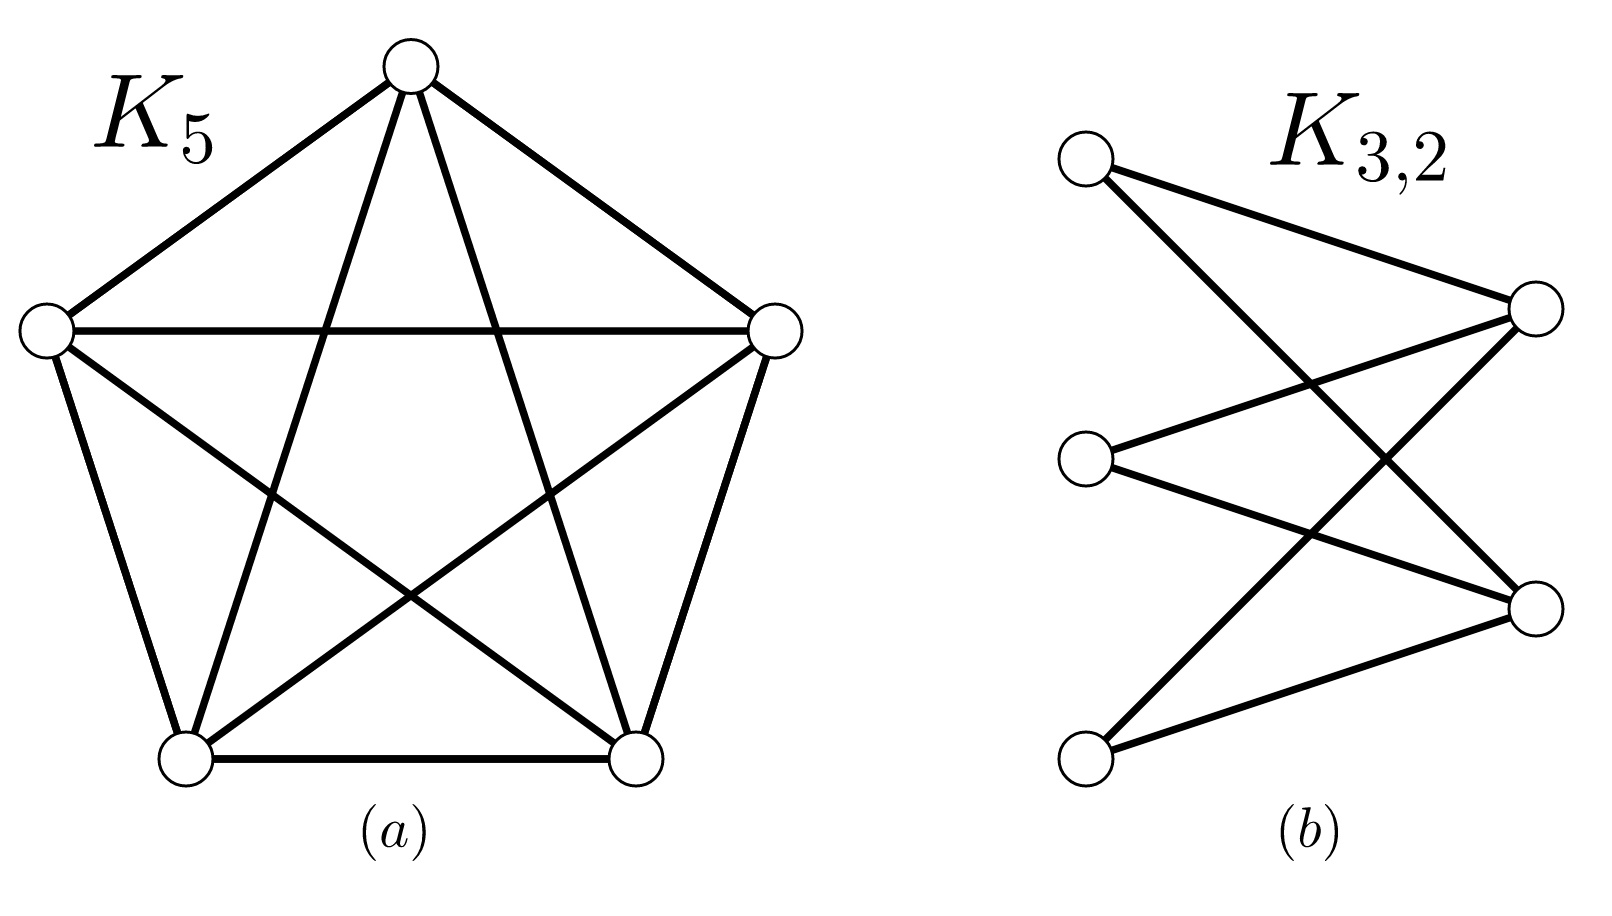
\includegraphics[scale=0.2]{img/imgchapter1/GrafosCompletos.jpg}
    \caption{}
    \label{fig:grafoscompletos}
\end{figure}

Una \textit{gráfica conexa} \index{Gráfica! conexa} es aquella en la que dada cualquier partición $(X,Y)$ de su conjunto de vértices, siempre hay al menos una arista con un extremo en $X$ y otro en $Y$. Si sucediera lo contrario, es decir, que exista una partición de sus vértices en los que no hay aristas entre tales conjuntos, entonces decimos que la gráfica no es conexa (o \textit{inconexa}).\index{Gráfica! inconexa}

La definición clásica de \textit{ciclo}\index{Ciclo} nos dice que es una gráfica conexa en la que todos sus vértices tienen grado $2$. La notación que suele utilizarse es $C_{n}$, donde $n$ es el número de vértices del ciclo; y es fácil notar que también debe tener $n$ aristas. A este número $n$ se le conoce como la \textit{longitud}\index{Longitud! de un ciclo} del ciclo. Así, bajo esta definición, un ciclo de longitud $1$ es, necesariamente, un lazo; y uno de longitud $2$ consta de un par de aristas paralelas. Véase la figura \ref{fig:ciclos}. 

\begin{figure}[h]
    \centering
    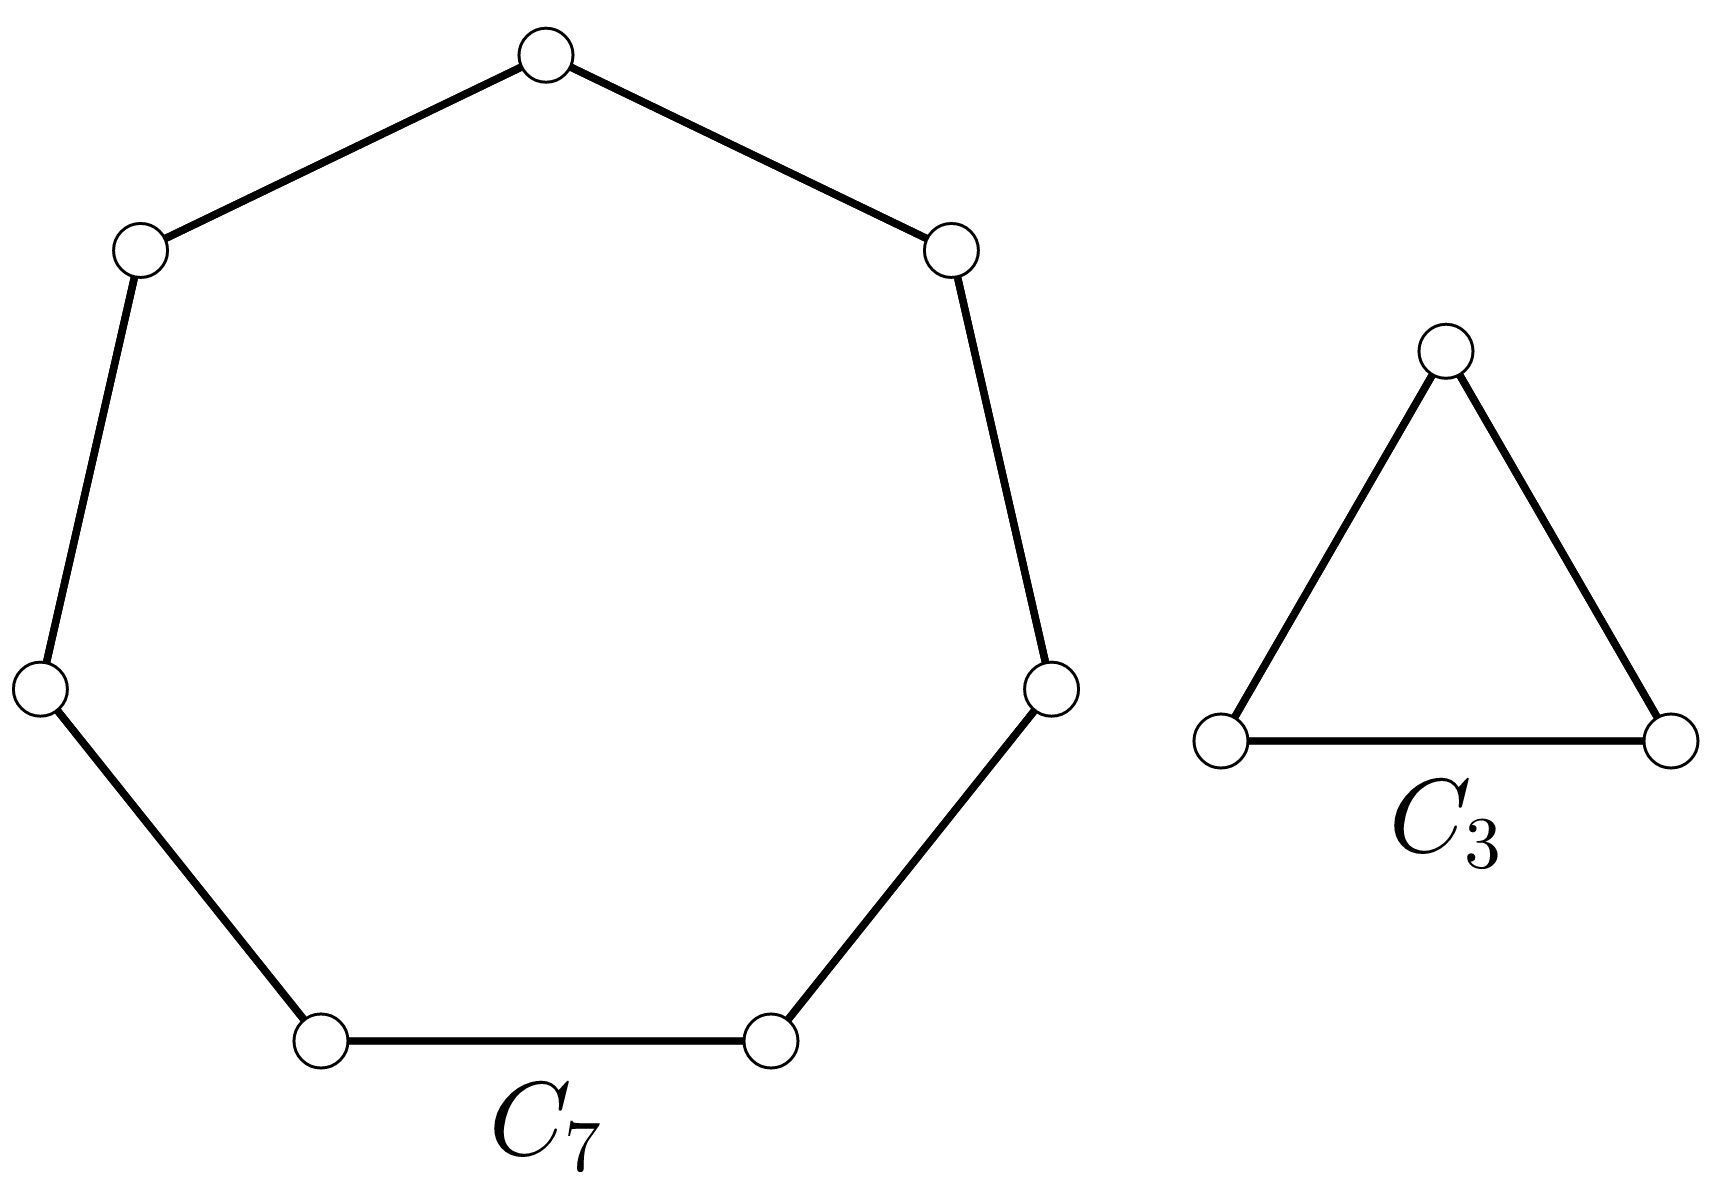
\includegraphics[scale=0.15]{img/imgchapter1/Ciclos.jpg}
    \caption{}
    \label{fig:ciclos}
\end{figure}

%Decimos que $u_{1}, \ldots, u_{n}$ ($n \geq 3$) forman un \textit{ciclo} si $u_{i}$ es %adyacente a $u_{i+1}$, con $i \in \{1, \ldots, n-1 \}$ y $u_{n}$ es adyacente a $u_{1}$. 
Los ciclos y su longitud son bastante útiles para caracterizar ciertas gráficas. Hechos tales como: que \textit{un ciclo es bipartito si y sólo si es de longitud par}; y que \textit{una gráfica es bipartita si y sólo si no contiene ciclos de longitud impar}, son ampliamente usados en la Teoría de Gráficas.

De hecho, el siguiente teorema nos será de mucha ayuda, pues ofrece condiciones necesarias para la existencia de ciclos.

%\renewcommand{\labelenumi}{\textnormal{\alph{enumi})}}
\begin{teo} \label{teo:ciclos}  
Si $G$ es una gráfica en la que todos sus vértices tienen grado al menos dos, entonces $G$ contiene un ciclo.
\end{teo}

\begin{teo} \label{teo: ciclos2}
Si $G$ es una gráfica con $n$ vértices y $m$ aristas, de tal manera que $m \geq n$ (o sea, que hay más aristas que vértices), entonces $G$ contiene un ciclo.
\end{teo}


        \subsection{Conexidad} \label{sec:conexidad}
 
Un \textit{camino} \index{Camino} en una gráfica $G$ es una sucesión $W:= u_{0}e_{1}u_{1}\ldots u_{l-1}e_{l}u_{l}$ de vértices y aristas de tal forma que $u_{i-1}$ y $u_{i}$ son extremos de $e_{i}$, con $i\in\{1, \ldots, l\}$. Los vértices y aristas que aparecen en $W$ no son necesariamente distintos. La \textit{longitud} \index{Longitud! de un camino} $W$ es la cantidad de aristas empleadas en el camino $W$ (también se cuentan las aristas repetidas).


\begin{ejem} \label{ejem:caminos}
Consideremos la gráfica $G$ con vértices $\{u_{1}, \ldots, u_{5}\}$ y aristas $\{e_{1}, \ldots, e_{7}\}$, como se muestra en la figura \ref{fig:GrafoCaminos}.
Entonces $W_{1}=u_{3}e_{5}u_{4}e_{5}u_{3}e_{3}u_{2}$, $W_{2}=u_{3}e_{4}u_{3}e_{5}u_{4}e_{6}u_{5}$ y $W_{3}=u_{5}e_{7}u_{4}e_{6}u_{5}e_{7}u_{4}e_{5}u_{3}e_{2}u_{1}$ son caminos en $G$. 

\begin{figure}[H]
    \centering
    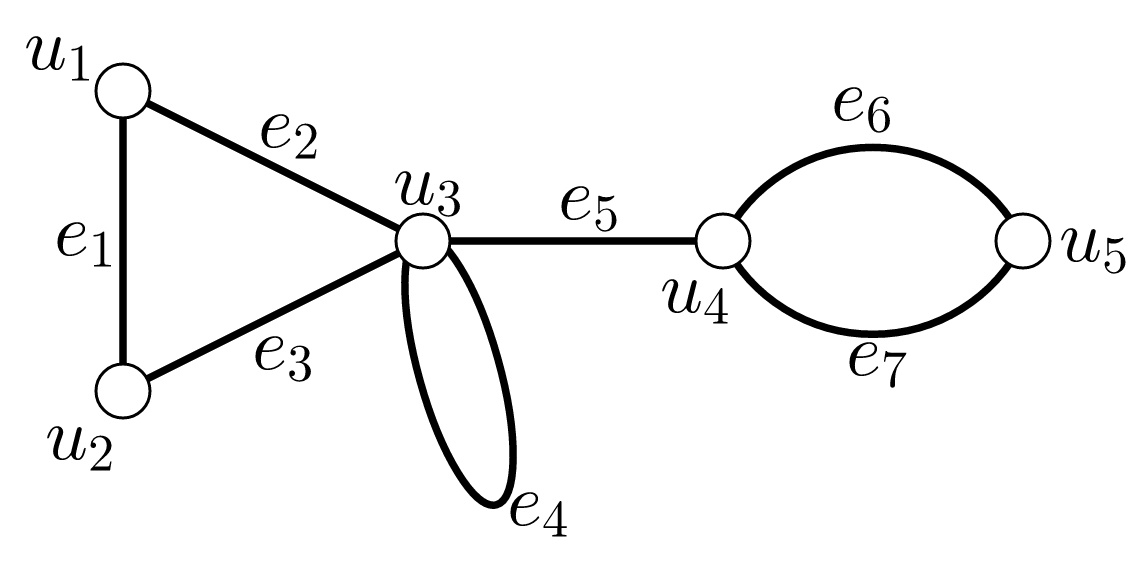
\includegraphics[scale=0.3]{img/imgchapter1/GrafoCaminos.jpg}
    \caption{}
    \label{fig:GrafoCaminos}
\end{figure}

\hfill $\blacklozenge$
\end{ejem}


Si $x = u_{0}$ y $y = u_{l}$, entonces decimos que $W$ es un $xy-camino$ y que $x$ y $y$ son los \textit{extremos}\index{Vértice! extremo} de $W$, los demás son vértices \textit{internos}\index{Vértice! interno}; suele emplearse la notación $xWy$. También se dice que $W$ \textit{conecta} a los vértices $x$ y $y$. Cuando las gráficas sean simples, los caminos se describen en términos de sus vértices, es decir, se omiten las aristas.


\begin{ejem}
El camino $W_{1}$ del ejemplo \ref{ejem:caminos} es un $u_{3}u_{2}-camino$ y su longitud es igual a $3$ porque utiliza las aristas $e_{5}$ (dos veces) y $e_{3}$.

El camino $W_{2}$ es un $u_{3}u_{5}-camino$ de longitud $3$ y $W_{3}$ es un $u_{5}u_{1}-camino$ de longitud $5$.


\hfill $\blacklozenge$
\end{ejem}


\begin{wrapfigure}{l}{0.35\textwidth}
%\vspace{-1.2cm}
\centering
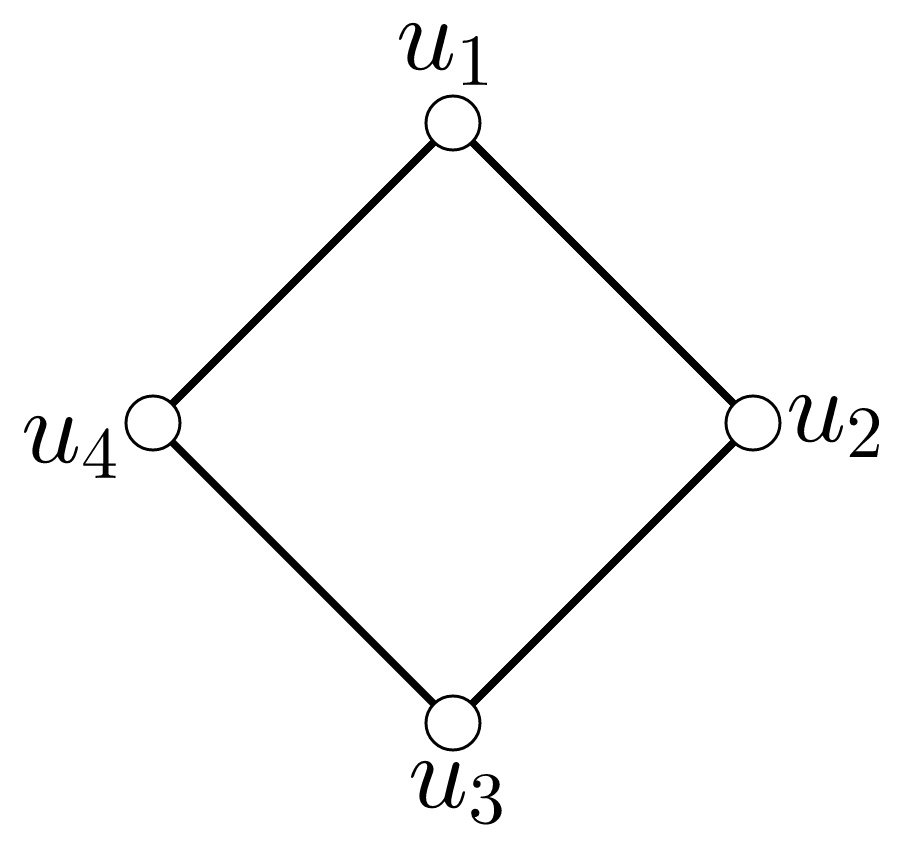
\includegraphics[scale=0.2]{img/imgchapter1/GrafoCiclo.jpg}
\caption{}
\label{fig:cicloc4}
\vspace{-0.5cm}
\end{wrapfigure}
Los caminos se clasifican dependiendo de las características de sus vértices y aristas. En efecto, decimos que un camino es \textit{cerrado} \index{Camino! cerrado} si sus extremos coinciden; si no, es \textit{abierto}. \index{Camino! abierto} Un \textit{paseo} \index{Paseo} es un camino en el que todas sus aristas son distintas (pero puede repetir vértices); y una \textit{trayectoria} \index{Trayectoria} es un camino en el que todos sus vértices son diferentes (y, por tanto, sus aristas también). 


Un $xy-paseo$ es un paseo cuyos extremos son los vértices $x$ y $y$. Una $xy-trayectoria$ se define análogamente. Además, cuando un paseo es cerrado (es decir, sus extremos son iguales) lo llamamos \textit{circuito}. \index{Circuito} La gráfica inducida por los vértices de un circuito, en el que todos sus vértices internos son distintos, es un ciclo.

De manera inversa, a cada ciclo podemos asignarle un circuito, aunque no de manera única. Para convencerse de esto, consideremos el ciclo $C_{4}$ de la figura \ref{fig:cicloc4}. Es claro que tanto $\Gamma_{1} = u_{1}u_{2}u_{3}u_{4}$ como $\Gamma_{2} = u_{4}u_{3}u_{2}u_{1}$ son dos circuitos que describen el mismo ciclo $C_{4}$. 

No obstante, será común que, cuando hablemos de ciclos, lo hagamos considerando alguno de sus circuitos asociados y referirnos a dicho circuito como el ciclo en sí. 

\begin{ejem}
Considerando ahora la gráfica \ref{fig:GrafoCaminos2}, es sencillo notar que un camino cerrado es $W_{1}=u_{1}u_{2}u_{6}u_{2}u_{1}$. 
 \begin{figure}[H]
    \centering
    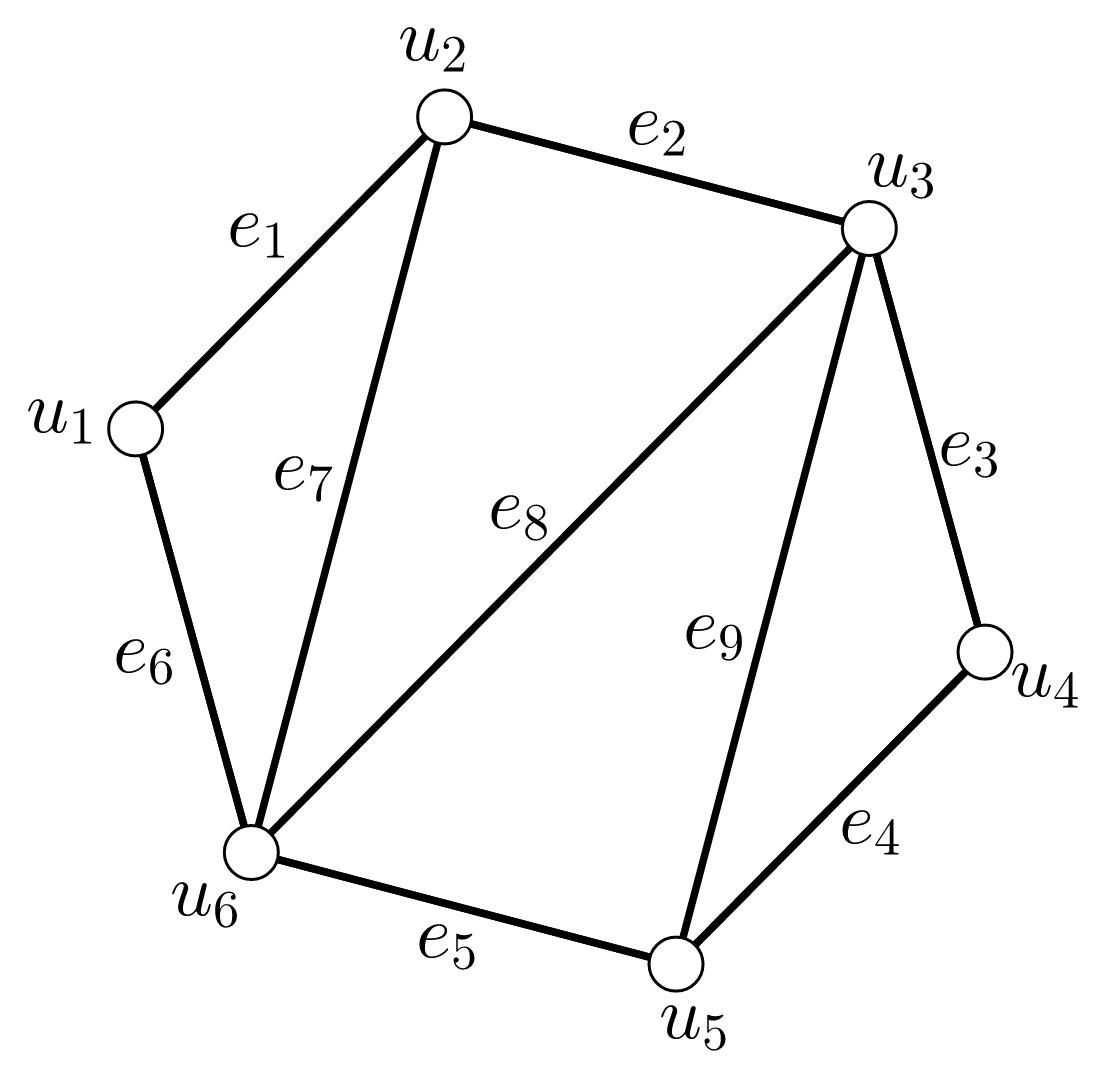
\includegraphics[scale=0.22]{img/imgchapter1/GrafoCaminos2.jpg}
    \caption{}
    \label{fig:GrafoCaminos2}
\end{figure}
Un paseo y una trayectoria serían $W_{2}=u_{5}e_{4}u_{4}e_{3}u_{3}e_{9}u_{5}e_{5}u_{6}e_{7}u_{2}$ y $W_{3} = u_{1}u_{2}u_{3}u_{4}$, respectivamente. Mientras que un circuito es $W_{4}=u_{2}u_{6}u_{3}u_{5}u_{4}u_{3}u_{2}$ y $W_{5}=u_{3}u_{4}u_{5}$ es un ciclo.

\hfill $\blacklozenge$
\end{ejem}

Se sabe bien que \textit{todo $uv-camino$ cerrado contiene un ciclo}. Más aún, \textit{que todo $uv-camino$ contiene una $uv-trayectoria$}. Estos nuevos conceptos nos permiten dar una nueva definición de conexidad, totalmente equivalente a la que dimos al principio. Efectivamente, una gráfica $G$ es \textit{conexa} si y sólo si, para cualquier par de vértices $u$ y $v$, existe una $uv-trayectoria$. Ambas versiones de la definición de conexidad serán usadas indistintamente a lo largo de este trabajo.

        \subsection{Operaciones en gráficas}
Hay varias \textit{operaciones} que se pueden realizar entre gráficas. A continuación, se detallan aquellas que más se usaremos en este trabajo.

Dadas dos gráficas $G$ y $H$, su \textit{unión}\index{Unión de gráficas} $G \cup H$ es la gráfica cuyos conjuntos de vértices y aristas son, respectivamente, $V(G) \cup V(H)$ y $E(G) \cup E(H)$. Su \textit{intersección}\index{Intersección de gráficas} $G \cap H$ tiene como vértices y aristas $V(G) \cap V(H)$ y $E(G) \cap E(H)$, respectivamente. La \textit{diferencia simétrica} de $G$ y $H$ está determinada por la diferencia simétrica de sus aristas, o sea, es la gráfica $G \triangle H$ con $V(G) \cup V(H)$ como conjunto de vértices y $E(G)\triangle E(H)$. Véase la figura \ref{fig:operaciones}.

\begin{figure}[H]
    \centering
    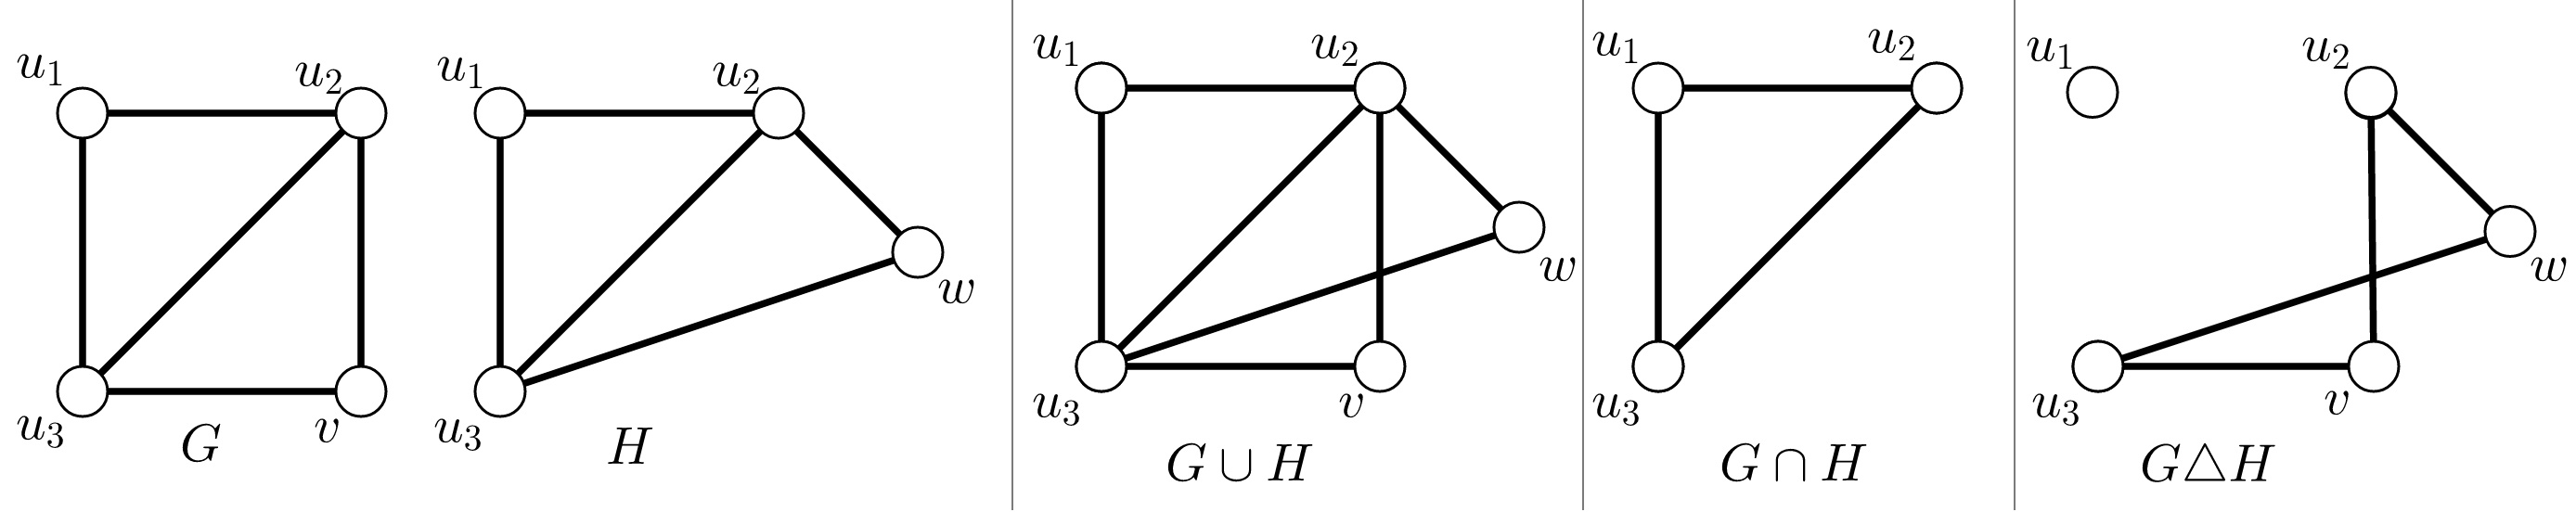
\includegraphics[scale=0.22]{img/imgchapter1/Operaciones.jpg}
    \caption{}
    \label{fig:operaciones}
\end{figure}

Diremos que $G$ y $H$ son \textit{ajenas} \index{Gráficas ajenas} si no tienen vértices en común, es decir, $V(G)\cap V(H) = \emptyset$. También decimos que son \textit{ajenas por aristas}\index{Gráficas ajenas por aristas} si $E(G)\cap E(H)=\emptyset$. De esta manera, si $G$ y $H$ son ajenas (o ajenas por aristas), decimos que $G \cup H$ es una \textit{unión ajena} (o \textit{ajena por aristas}). \index{Unión de gráficas ajenas} 

Si una gráfica es inconexa, entonces puede expresarse como una unión ajena de gráficas conexas, las cuales llamamos \textit{componentes conexas}\index{Componentes conexas}. A la cantidad total de componentes conexas de una gráfica $G$ se le denota por $c(G)$. Si $G$ es conexa, entonces $c(G)=1$.

Si $e \in E(G)$, entonces $G\setminus e$ es la gráfica que resulta de remover la arista $e$ de $G$ (conservando los vértices). Si $S\subseteq E(G)$, $G\setminus S$ se define de manera análoga. Si $e$ es una arista con extremos en $V(G)$, que no pertenece a $E(G)$, la gráfica $G+e$ es aquella que añade $e$ a la gráfica $G$. Similarmente, se define $G + S$, donde $S$ es un conjunto de aristas que no están en $E(G)$ y sus extremos son vértices de $G$.


        \subsection{Bosques y árboles} \label{sec:arboles}
\begin{wrapfigure}{r}{0.42\textwidth}
\vspace{-1cm}
 \centering
  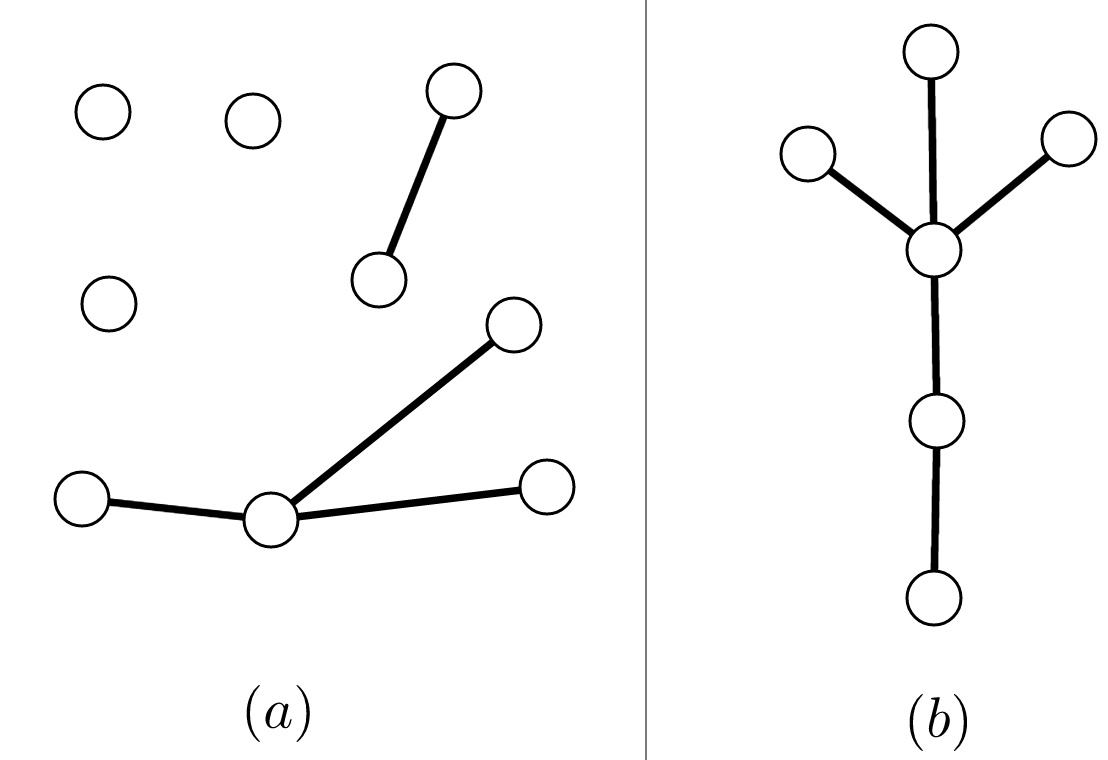
\includegraphics[scale=0.25]{img/imgchapter1/arboles.jpg}
  \caption{}
  \label{fig:arboles}
\end{wrapfigure}
Un \textit{bosque}\index{Bosque} es una gráfica sin ciclos (\textit{acíclica}). Si un bosque es conexo, se le dice \textit{árbol}. \index{\'{A}rbol} Luego, un árbol es una gráfica conexa sin ciclos. Se desprende de aquí que las componentes conexas de los bosques son, precisamente, árboles. Un  árbol que consta de un sólo vértice es un \textit{árbol trivial}. En caso contrario, es \textit{no trivial}. Desde luego, un \textit{bosque trivial} se compone de árboles triviales. 

Los árboles son la columna vertebral de las gráficas. Su importancia es enorme  debido a sus aplicaciones. Varios resultados provienen de este concepto. De hecho, jugarán un papel clave en esta tesis. En lo que sigue mencionaremos algunas de sus propiedades.

\begin{prop}\label{prop:treepath}
Dos vértices cualesquiera en un árbol están conectados por una única trayectoria.
\end{prop}

En virtud de la contrapositiva del teorema \ref{teo:ciclos}, todo bosque tiene un vértice de grado a lo más igual a uno. Aún más:

\begin{prop} \label{prop:hojas}
Todo árbol no trivial tiene al menos dos vértices de grado uno. En general, todo bosque no trivial también tendrá al menos dos vértices de grado uno. 
\end{prop}

 En un bosque son \textit{hojas} los vértices que tienen grado uno. Así, la proposición \ref{prop:hojas} nos garantiza que cualquier árbol no trivial tendrá al menos dos hojas. La contrapositiva del teorema \ref{teo: ciclos2} asegura que en un bosque hay más vértices que aristas. El teorema que sigue es crucial en el desarrollo de este trabajo: nos da la cantidad exacta de aristas de un árbol.

\begin{teo} \label{teo:tree}
Si $T$ es cualquier árbol, entonces $|E(T)| = |V(T)|-1$. 
\end{teo}

Suponiendo que $G$ es una gráfica conexa, las subgráficas generadoras de $G$, que al mismo tiempo son árboles, reciben el nombre de \textit{árboles generadores}. \index{\'{A}rbol! generador} De hecho, \textit{cualquier gráfica $G$ es conexa si y sólo si $G$ contiene un árbol generador}.  Por supuesto, si $G$ es inconexa, sus subgráficas generadoras acíclicas son \textit{bosques generadores}.\index{Bosque! generador} Los \textit{bosques generadores maximales} de $G$ son aquellos que no están contenidos en ningún otro bosque generador y, por lo tanto, sus componentes conexas son árboles generadores de cada componente conexa de $G$ (si $G$ es conexa, sus bosques generadores maximales son simplemente sus árboles generadores).

Del teorema \ref{teo:tree}, obtenemos el siguiente resultado:

\begin{teo}
Si $G$ tiene $n$ vértices, sus bosques generadores maximales constan necesariamente de $n-c(G)$ aristas. En particular, si $G$ es conexa, sus árboles generadores poseen $n-1$ aristas.
\end{teo}


        \subsection{Matriz de incidencia de una gráfica} \label{sec:matriz}
Sea $G$ una gráfica cualquiera con $n$ vértices y $m$ aristas. La \textit{matriz de incidencia de} $G$ \index{Matriz! de incidencia de una gráfica}es la matriz $\mathbf{M}_{G} := [m_{ve}] \in \mathbb{M}_{n \times m}(\mathbb{R})$, donde

$$ m_{ve}=
\begin{cases}
0, & \text{si el vértice } v \text{ no es adyacente a la arista } e \\ 
1, & \text{si } v \text{ es adyacente a } e\\ 
2, & \text{si } e \text{ es un lazo en } v
\end{cases}
$$

En la figura \ref{fig:matrizdeincidencia} mostramos una gráfica y su matriz de incidencia.

\begin{figure}[H]
    \centering
    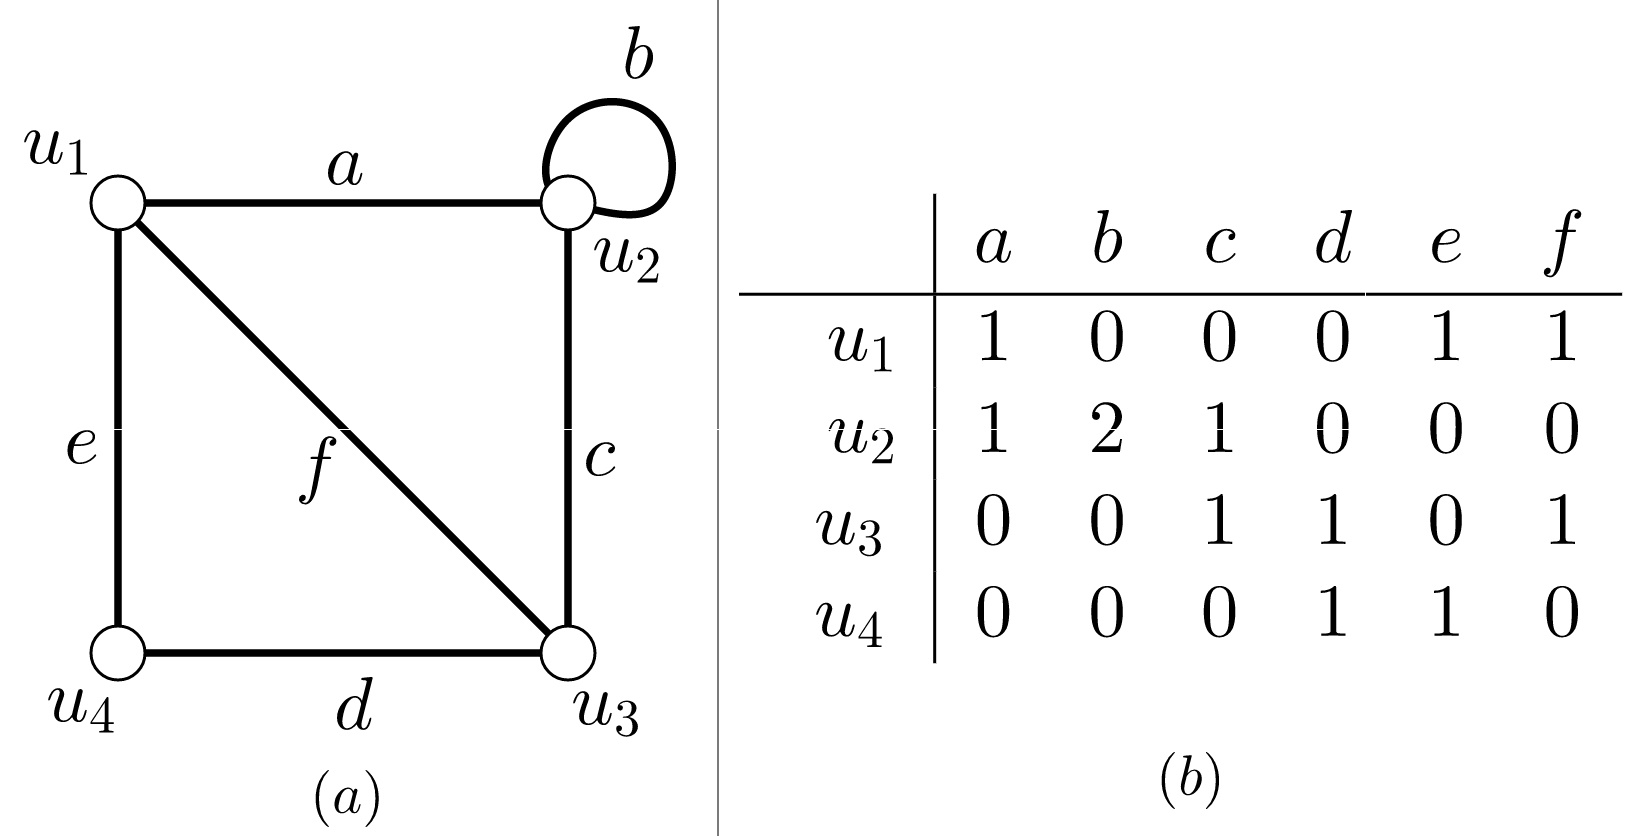
\includegraphics[scale=0.25]{img/imgchapter1/matrizdeincidencia.jpg}
    \caption{}
    \label{fig:matrizdeincidencia}
\end{figure}

Supongamos que $G$ es inconexa y digamos que sus componentes conexas son $F_{1}, \ldots, F_{k}$. Dado que los vértices entre diferentes componentes no son adyacentes, se tiene que la matriz de incidencia de $G$ es una matriz diagonal por bloques, donde cada bloque corresponde a la matriz de incidencia de cada componente (siempre y cuando los vértices y las aristas estén etiquetados de manera ordenada) (véase el ejemplo \ref{ejem:matrizDeIncidenciaDeInconexa} ):

$$
\mathbf{M}_{G}=\begin{bmatrix}
\mathbf{M}_{F_{1}} & \cdots  & \mathbf{O}\\ 
\vdots & \ddots & \vdots\\ 
\mathbf{O} & \cdots & \mathbf{M}_{F_{k}}
\end{bmatrix}.
$$

\begin{ejem}\label{ejem:matrizDeIncidenciaDeInconexa}
Considere la gráfica $G$ de la siguiente figura.

\begin{figure}[H]
    \centering
    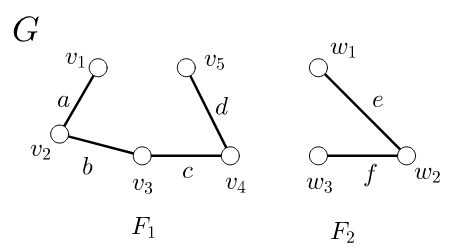
\includegraphics[scale=0.75]{img/imgchapter1/matrizDeIncidenciaInconexa.png}
    \caption{}
    \label{fig:matrizdeincidenciaInconexa}
\end{figure}

Entonces su matriz de incidencia es:
\begin{center}


$\mathbf{M}_{G} =$ \begin{tabular}{c| c c c c c c c }
 & $a$ & $b$ & $c$ & $d$ &    & $e$ & $f$\\
\hline \
$v_{1}$ & 1 & 0 & 0 & 0 & $|$ & 0 & 0\\ 
$v_{2}$ & 1 & 1 & 0 & 0 & $|$ & 0 & 0\\ 
$v_{3}$ & 0 & 1 & 1 & 0 & $|$ & 0 & 0\\ 
$v_{4}$ & 0 & 0 & 1 & 1 & $|$ & 0 & 0\\ 
$v_{5}$ & 0 & 0 & 0 & 1 & $|$ & 0 & 0\\
        & --& --& --& --& --  & --& --\\
$w_{1}$ & 0 & 0 & 0 & 0 & $|$ & 1 & 0  \\ 
$w_{2}$ & 0 & 0 & 0 & 0 & $|$ & 1 & 1 \\ 
$w_{3}$ & 0 & 0 & 0 & 0 & $|$ & 0 & 1  
\end{tabular} $= \begin{bmatrix}
\mathbf{M}_{F_{1}} & \mathbf{O}\\ 
\mathbf{O} & \mathbf{M}_{F_{2}}
\end{bmatrix}. $
\end{center}
\hfill $\blacklozenge$
\end{ejem}

$\mathbf{M}_{G}$ es una matriz que tiene tantos renglones como vértices hay en $G$, y tantas columnas como aristas. Cada una de sus entradas indica qué ``tipo'' de adyacencia hay entre el vértice (renglón) y la arista (columna) correspondientes.  

De lo anterior, es sencillo observar que si tomamos cualquiera de sus renglones, la suma de todas sus entradas es igual al grado del vértice asociado. En otras palabras: que $\sum_{e \in E(G)}m_{ve} = d(v)$, con $v$ un vértice fijo.

De igual modo, considerando una columna cualquiera, la suma de todos sus renglones es $2$, pues la arista correspondiente es adyacente, a lo más, en dos vértices (recordemos que si la arista es un lazo, es adyacente a un único vértice cuyo grado sería $2$). Luego, $\sum_{v \in V(G)}m_{ve} = 2$, con $e$ una arista fija.

La demostración del siguiente teorema (que se mencionó antes) es un primer vistazo de la utilidad y del potencial que la matriz de incidencia posee para representar y estudiar (desde otros puntos de vista) propiedades de las gráficas. En los capítulos siguientes desarrollaremos estas ideas.


\begin{teo}
En cualquier gráfica $G$, se cumple que

$$
\sum_{v \in V(G)} d(v) = 2 \cdot|E(G)|. 
$$
\end{teo}

\begin{proof}
Es un hecho conocido que la suma total de todas las entradas de una matriz puede obtenerse de dos formas: sumando las entradas columna por columna, o bien sumando las entras renglón por renglón. Esto, respecto a la matriz de incidencia, se traduce en la siguiente igualdad:

$$
\sum_{v \in V(G)} (\sum_{e \in E(G)} m_{ve}) = \sum_{e \in E(G)} (\sum_{v \in V(G)} m_{ve}).
$$
Considerando lo dicho en párrafos anteriores:

$$
\sum_{v \in V(G)} d(v) = \sum_{e \in E(G)} 2.
$$

Así, concluimos que la suma de los grados de todos los vértices de $G$ es igual al doble de sus aristas, o sea, $\sum_{v \in V(G)} d(v) = 2 |E(G)|$.

\end{proof}

        \subsection{Digráficas} \label{sec:queesunadigrafica}

Una \textit{digráfica} \index{Gráfica! dirigida} $D$ (también llamada \textit{gráfica dirigida} \index{Digráfica}) es un par ordenado $(V(D), A(D))$, donde $V(D)$ es el conjunto de \textit{vértices}\index{Vértice! de una digráfica} de $D$, y $A(D)$ (ajeno con $V(D)$) su conjunto de \textit{arcos}\index{Arco de una digráfica}; junto con una \textit{función de incidencia} \index{Función de incidencia! de una digráfica}
 $\psi_D \colon A(D) \rightarrow V(D) \times V(D)$ que asigna a cada arco de la digráfica un par ordenado de vértices (no necesariamente diferentes).
 
 Tomando un arco $a$ cualquiera, y suponiendo que $\psi_D (a) = (u,v)$, diremos que $u$ y $v$ son extremos del arco $a$ y que éste \textit{une} a $u$ con $v$ o, mejor dicho, que $u$ \textit{domina} a $v$. También decimos que $u$ es la \textit{cola} \index{Vértice! cola} de $a$ y $v$ su \textit{cabeza} \index{Vértice! cabeza}, y escribimos $t(a) = u$ y $h(a)=v$, respectivamente.
 
 Igual que en las gráficas, solemos representar las digráficas con diagramas \index{Diagrama! de una digráfica} y pensar que éstos son las digráficas en sí. La diferencia aquí es que los arcos se dibujan como flechas entre sus vértices extremos, para indicar la ``dominancia'' entre ellos. Entonces, las flechas ``salen'' de las colas de los arcos y ``entran'' en la cabeza (la punta de la flecha) de los mismos (ver figura \ref{ejem:diagramadigrafica}).
 
 Por otro lado, también se suele no escribir la letra ``$D$'' de los símbolos que representan los conjuntos de vértices y arcos, y omitir la función de incidencia (quedando sobreentendida con el diagrama empleado).
 
 El \textit{ingrado}\index{Ingrado} de $v$, $d_{D}^{-}(v)$, es la cantidad de arcos cuya cabeza es $v$. Similarmente, a la cantidad de arcos cuya cola es $v$ es el \textit{exgrado}\index{Exgrado} de $v$, denotado como $d_{D}^{+}(v)$. El \textit{grado}\index{Grado} de $v$ es sencillamente la suma de su exgrado y su ingrado, es decir, $d_{D}(v) : = d_{D}^{+}(v) + d_{D}^{-}(v)$. Un \textit{pozo} es un vértice de exgrado igual a cero y una \textit{fuente} uno de ingrado igual a cero.
 
 \begin{ejem} \label{ejem:diagramadigrafica}
 Consideremos la digráfica $D = (V(D),A(D))$, con $V(D)=\{u_{1}, u_{2},u_{3},u_{4}\}$ y \\ $E(G)=\{a,b,c,d,e,f,g\}$, y $\psi_{D}$ definida como sigue:

\begin{center}
\begin{tabular}{ c c c c }
$\psi_{D}(a) = (u_{2},u_{1})$& $\psi_{D}(b) = (u_{1},u_{2})$ & $\psi_{D}(c) = (u_{2},u_{3})$ & $\psi_{D}(d) = (u_{3},u_{4})$  \\
$\psi_{D}(e) = (u_{1},u_{4})$  & $\psi_{D}(f) = (u_{1},u_{5})$ & $\psi_{D}(g) = (u_{5},u_{5})$
\end{tabular}
\end{center}

El diagrama que representa a $D$ se muestra en la figura \ref{fig:digraficadiagrama}. En particular, el ingrado de $u_{1}$ es igual a $1$ y su exgrado es $3$. Obsérvese que $d^{-}(u_{2})=1$ y que $u_{4}$ es un pozo pues $d^{+}(u_{4})=0$. Nótese además que la cola del arco $d$ es $u_{3}$ y su cabeza es $u_{4}$. De igual modo, $t(f) = u_{1}$ y $h(f)=u_{5}$.
\begin{figure}[H]
    \centering
    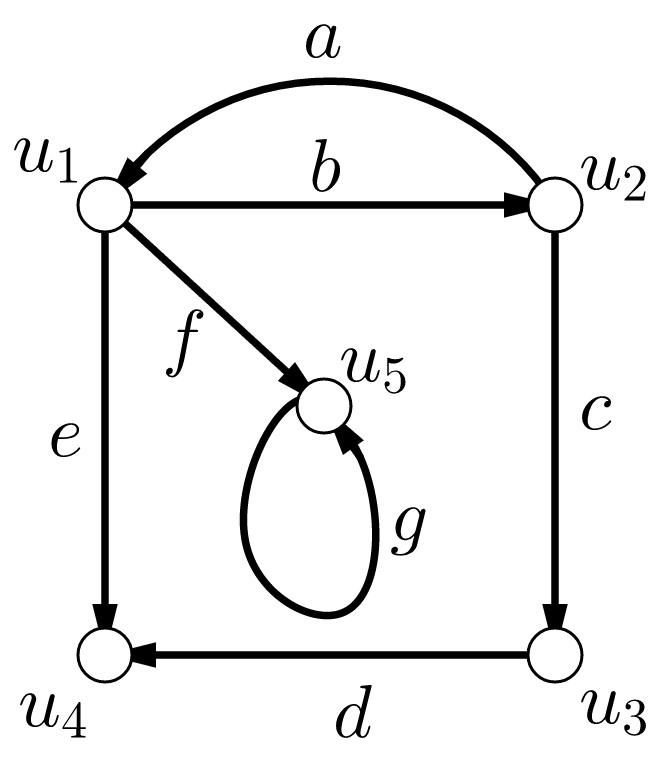
\includegraphics[scale=0.3]{img/imgchapter1/digrafica.jpg}
    \caption{Diagrama de una digráfica}
    \label{fig:digraficadiagrama}
\end{figure}

\hfill $\blacklozenge$
 \end{ejem}
 %De igual modo, tomando $v$ en $V(D)$, se le llama \textit{invecino} a cualquier vértice %que domina a $v$; y \textit{exvecino} a cualquier vértice dominado por $v$. Escribimos %$N_D^{-} (v)$ al conjunto de invecinos de $v$, y $N_D^{+} (v)$ a su conjunto de %exvecinos.
 
 
        \subsection{Algunas digráficas, conexidad y matriz de incidencia}
 A partir de una digráfica $D$ cualquiera, podemos obtener la \textit{gráfica subyacente de} $D$, \index{Gráfica! subyacente} denotada como $G(D)$. Tal gráfica se obtiene de reemplazar los arcos de $D$ por aristas con los mismos extremos. En la figura \ref{fig:subyacente} se muestra la gráfica subyacente de la digráfica del ejemplo \ref{ejem:diagramadigrafica}. Y si invertimos las orientaciones de sus arcos, obtendremos una nueva digráfica llamada \index{Converso de una digráfica} \textit{converso}.
 \begin{figure}[H]
 \centering
    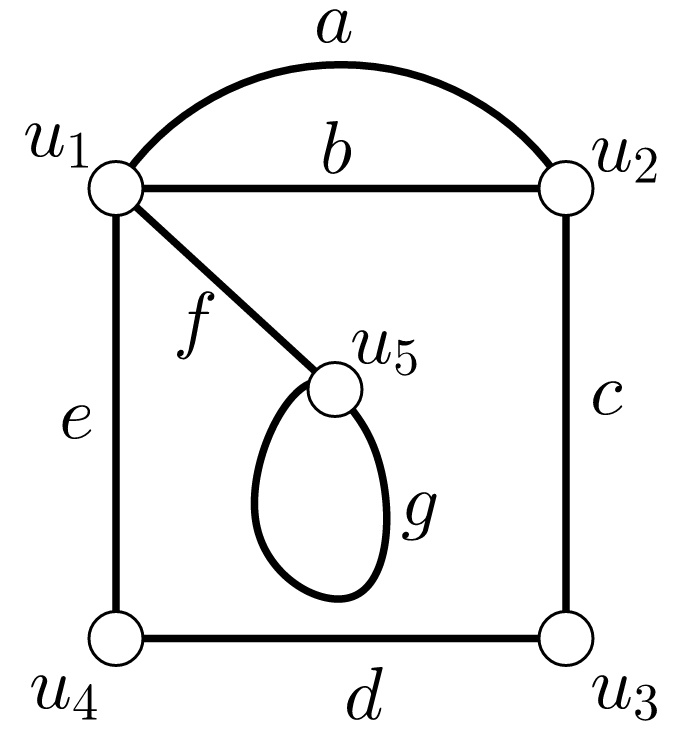
\includegraphics[scale=0.25]{img/imgchapter1/graficasubyacente.jpg}
    \caption{}
    \label{fig:subyacente}
 \end{figure} 
De una gráfica $G$ es posible construir una digráfica ``orientando'' \index{Orientación de una gráfica} sus aristas, es decir, reemplazando cada arista por uno de los dos posibles arcos entre sus extremos. Tal digráfica se le conoce como \textit{orientación de} $G$, y la escribimos $\overrightarrow{G}$. Debe notarse que una gráfica puede tener varias orientaciones.


Muchos de los conceptos \index{Subdigráfica} \index{Ciclo! de una digráfica} \index{\'{A}rbol! de una digráfica} \index{Bosque! de una digráfica} en digráficas son similares a los de las gráficas no dirigidas. Por ejemplo, la definición de  \textit{subdigráfica} de un digráfica es análogo al de \textit{subgráfica}. Los ciclos, bosques y árboles de una digráfica son los mismos de su gráfica subyacente (pero conservando las orientaciones de los arcos). Véase la figura \ref{fig:ciclosdigrafica}. 

 \begin{figure}[H]
    \centering
    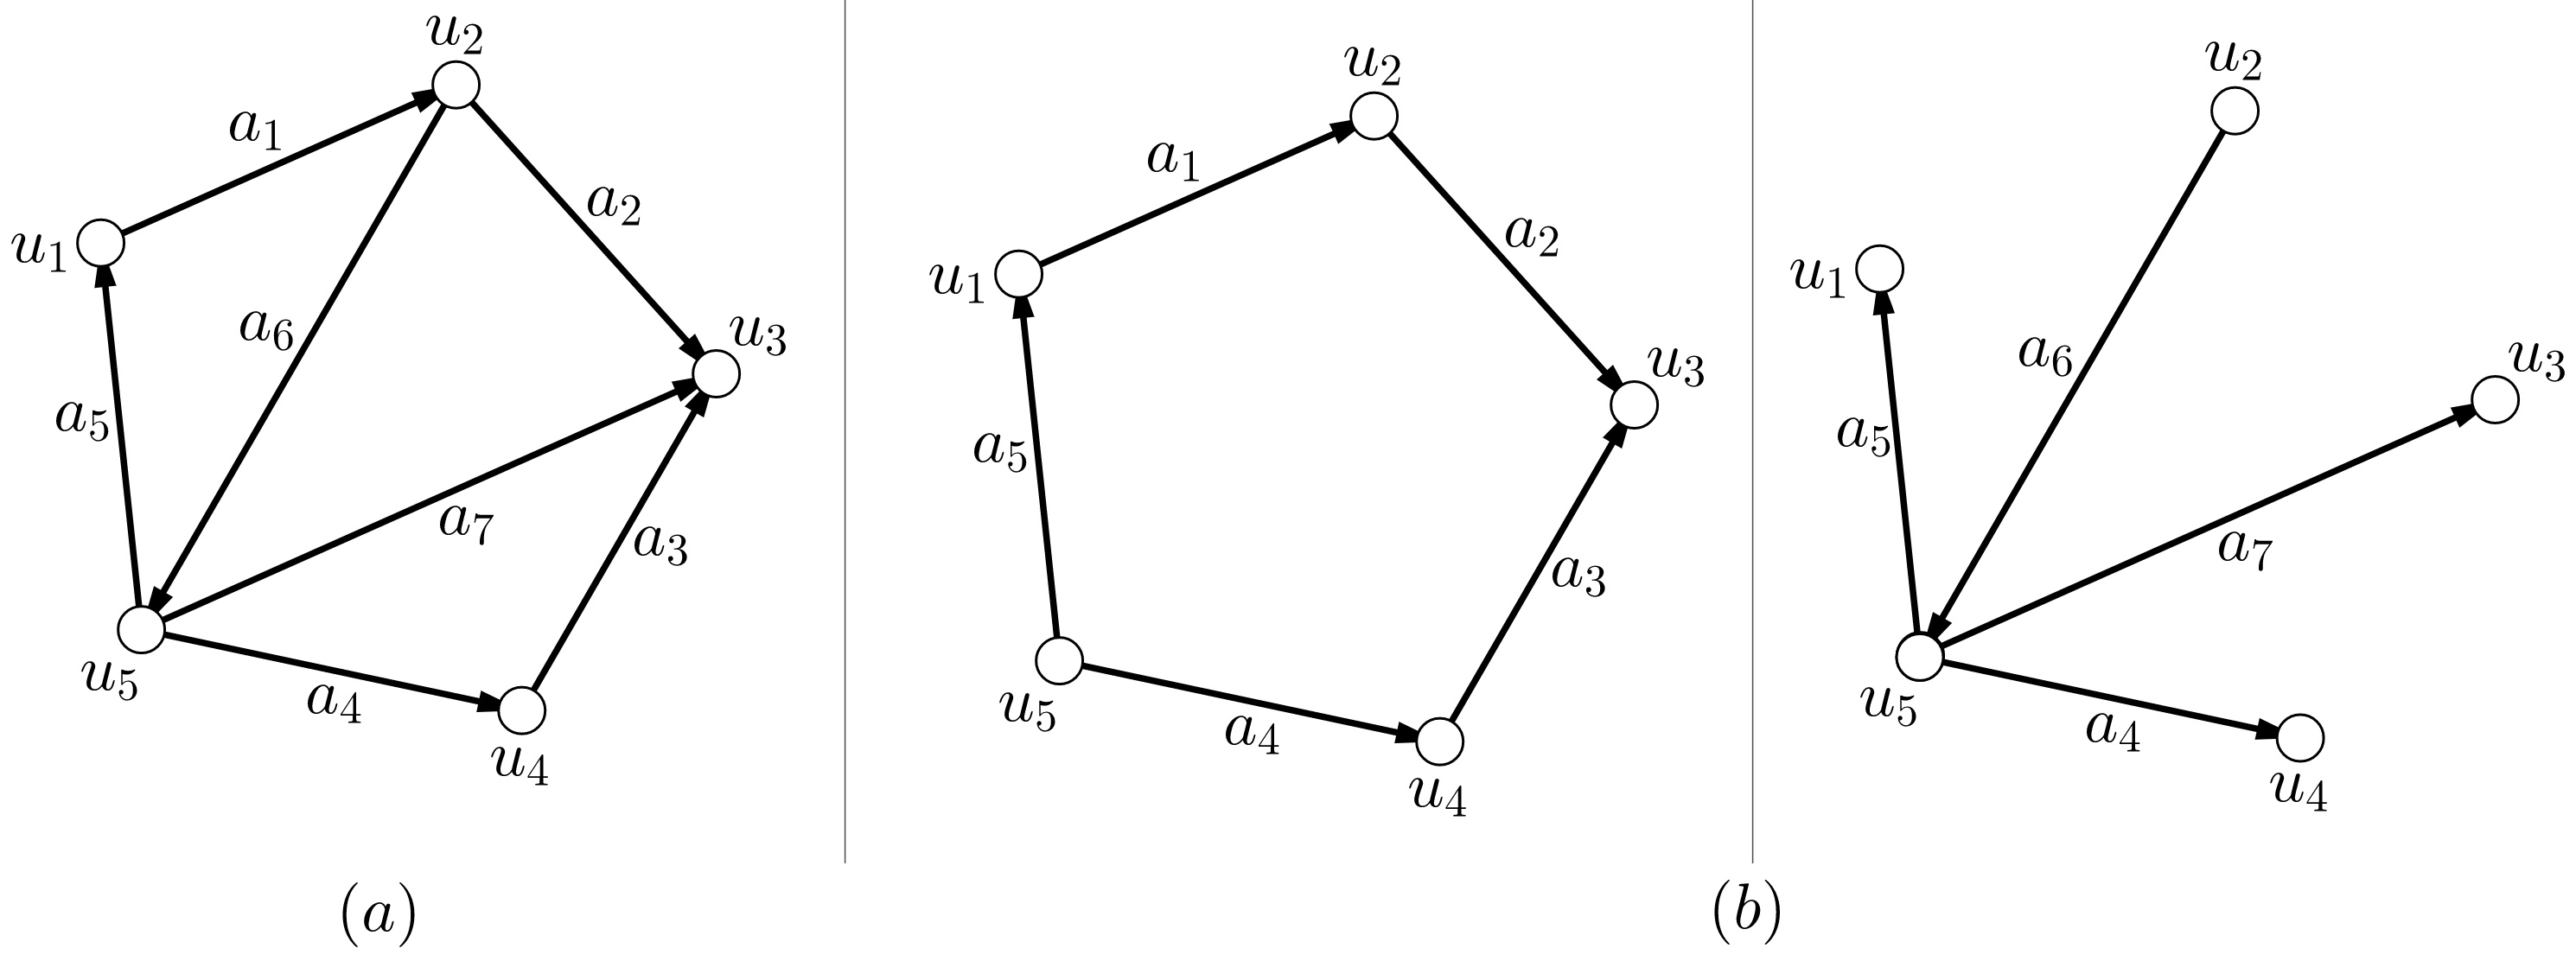
\includegraphics[scale=0.17]{img/imgchapter1/ciclosdigrafica.jpg}
    \caption{Ciclos y árboles en digráficas}
    \label{fig:ciclosdigrafica}
\end{figure}

Un \textit{camino} \index{Camino! de una digráfica} en una digráfica se define de manera análoga a las gráficas: es una sucesión \\$W:= u_{0}a_{1}u_{1}\ldots u_{l-1}a_{l}u_{l}$ de vértices y arcos de tal forma que $u_{i-1}$ y $u_{i}$ son extremos de $a_{i}$, con $i\in\{1, \ldots, l\}$. Sin embargo, hay que destacar que $u_{i-1}$ no necesariamente domina a $u_{i}$; si fuera el caso, se dice que el camino es \index{Camino! dirigido} \textit{dirigido}. La misma terminología para los caminos en gráficas se usa aquí y las trayectorias, paseos y circuitos también de definen \index{Paseo! de una digráfica} \index{Circuito! de una digráfica} \index{Trayectoria! de una digráfica} parecido. Retomando la digráfica de la figura \ref{fig:digraficadiagrama}, $W_{1} = u_{1}eu_{4}du_{3}cu_{2}$ y $W_{2}=u_{1}bu_{2}cu_{3}du_{4}$ son caminos, y $W_{3}= u_{1}bu_{2}au_{1}fu_{5}gu_{5}$ es un camino dirigido.

Una digráfica $D$ es \textit{conexa}\index{Digráfica! conexa} si su gráfica subyacente es conexa, y es \textit{fuertemente conexa} \index{Digráfica! fuertemente conexa} si, para cualquier par de vértices $x$ y $y$, de $D$, existen un $xy-camino$ y un $yx-camino$.  

Las gráficas dirigidas también tienen sus propias matrices de incidencia. Suponiendo que $D$ es una digráfica cualquiera con $n$ vértices y $m$ arcos, su \textit{matriz de incidencia}\index{Matriz! de incidencia de una digráfica} es la matriz $\mathbf{M}_{D}:= [m_{va}] \in \mathbb{M}_{n \times m}(\mathbb{R})$, donde
$$ m_{va}=
\begin{cases}
\quad \! 1, & \text{si el vértice } v \text{ es cola de } a \text{ y } a \text{ no es un lazo}\\ 
-1, & \text{si } v \text{ cabeza de } a \text{ y } a \text{ no es un lazo}\\ 
\quad \! 0, & \text{en otro caso}
\end{cases}
$$

Como es de esperarse, las matrices de incidencia de digráficas inconexas son también matrices diagonales por bloques, siempre y cuando los vértices y arcos estén etiquetados de manera ordenada.

\begin{ejem}
En la figura \ref{fig:matrizdeincidenciadigrafica} observamos la matriz de incidencia de una orientación de la gráfica de la figura \ref{fig:matrizdeincidencia}.
\begin{figure}[H]
    \centering
    \vspace{-0.8cm}
    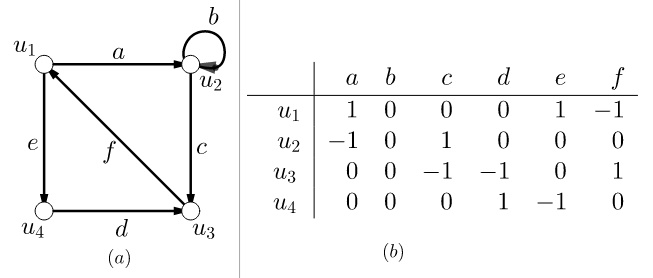
\includegraphics[scale=0.6]{img/imgchapter1/matrizDeIncidenciaDigrafica.jpg}
    \caption{}
    \label{fig:matrizdeincidenciadigrafica}
\end{figure}
\vspace{-0.5cm}
\hfill $\blacklozenge$
\end{ejem}







 